\documentclass [11pt,twoside]{article}
\usepackage[utf8]{inputenc}
\usepackage[T1]{fontenc}


%Page margins, header and footer positions
\usepackage{geometry}
 \geometry{
 a4paper,
 total={210mm,297mm},
 left=25mm,
 right=25mm,
 top=30mm,
 bottom=25mm,
 headsep=7mm}

\interfootnotelinepenalty=10000

%To display filling dots in the TOC for all entries
\usepackage[titles]{tocloft}
\renewcommand{\cftsecleader}{\cftdotfill{\cftdotsep}}

%Define new header and footer style
\usepackage{fancyhdr}

\pagestyle{fancy}
\fancyhf{}
\lhead{\color{Gray}{\small{}}}
\lfoot{\textcolor{Gray}{\small{}}}
\rfoot{\textcolor{Gray}{\thepage}}
\renewcommand{\headrulewidth}{0pt}

%PACKAGES
\usepackage{wasysym}
\usepackage{pifont}

\newcommand{\supported}{\ding{52}\xspace}
\newcommand{\unsupported}{\ding{55}\xspace}
\newcommand{\partsupported}{\textcolor{black!40}{\ding{52}}\xspace}
\newcommand{\lowsupported}{\textcolor{black!20}{\ding{52}}\xspace}
\newcommand{\unknowsupported}{\textbf{?}\xspace}

%Font: Times
\usepackage{times}
%Change monospaced font
\renewcommand{\ttdefault}{lmtt}

%tables
\usepackage{tabu}
\usepackage{tabularx}
\usepackage{ltablex}
\usepackage{longtable}
\usepackage{float} % To allow the use of H modifier in long tables

%landscape mode
\usepackage{pdflscape}
\usepackage{rotating}
\usepackage{caption}

% %make landscape mode be sensitive to even and odd pages
% %start
% \def\myrotate{\ifodd\c@page\else-\fi 90}
% \makeatletter
% \global\let\orig@begin@landscape=\landscape%
% \global\let\orig@end@landscape=\endlandscape%
% \gdef\@true{1}
% \gdef\@false{0}
% \gdef\landscape{%
%     \global\let\within@landscape=\@true%
%     \orig@begin@landscape%
% }%
% \gdef\endlandscape{%
%     \orig@end@landscape%
%     \global\let\within@landscape=\@false%
% }%
% \@ifpackageloaded{pdflscape}{%
%     \gdef\pdf@landscape@rotate{\PLS@Rotate}%
% }{
%     \gdef\pdf@landscape@rotate#1{}%
% }
% \let\latex@outputpage\@outputpage
% \def\@outputpage{
%     \ifx\within@landscape\@true%
%         \if@twoside%
%             \ifodd\c@page%
%                 \gdef\LS@rot{\setbox\@outputbox\vbox{%
%                     \pdf@landscape@rotate{-90}%
%                     \hbox{\rotatebox{90}{\hbox{\rotatebox{180}{\box\@outputbox}}}}}%
%                 }%
%             \else%
%                 \gdef\LS@rot{\setbox\@outputbox\vbox{%
%                     \pdf@landscape@rotate{+90}%
%                     \hbox{\rotatebox{90}{\hbox{\rotatebox{0}{\box\@outputbox}}}}}%
%                 }%
%             \fi%
%         \else%
%             \gdef\LS@rot{\setbox\@outputbox\vbox{%
%                 \pdf@landscape@rotate{+90}%
%                 \hbox{\rotatebox{90}{\hbox{\rotatebox{0}{\box\@outputbox}}}}}%
%             }%
%         \fi%
%     \fi%
%     \latex@outputpage%
% }
% \makeatother
% %end

%graphics
\usepackage{graphicx}
\usepackage[dvipsnames, table]{xcolor}
%If you upload images from PC, you need to insert code for the path here (different for Windows and Unix OS)

%References
%\usepackage{xpatch}
%\usepackage[backend=biber, style=numeric, citestyle=numeric, sorting=none]{biblatex}
%\addbibresource{main.bib}


%Other
\usepackage{ifthen}
\usepackage{xspace}
\usepackage{enumitem}
\usepackage{amssymb}
\usepackage[pdftex, colorlinks]{hyperref}


% added to define a cool blue color
\definecolor{myblue}{RGB}{85, 152, 192}

% added to change colors of links
\hypersetup{
    colorlinks=true,
    linkcolor=myblue,
    filecolor=magenta,      
    urlcolor=cyan,
    }

\newcommand{\comment}[1]{{\color{Red}$\blacktriangleright$ Comment: #1 $\blacktriangleleft$}}


% Some utilities\ldots
\input{util/highlight}
\input{util/abbrev}

\date{}


% Added by Leo to provide no hyphenation in the first cell of the table of definitions
\usepackage[none]{hyphenat}

% Added by Leo to reduce globally linespread between \item in \itemize environment
\setlist[1]{itemsep=-5pt}


% Added by Leo to introduce links in references
\usepackage{url}

% Added by Leo to introduce a new command for internal section references
\newcommand{\rref}[1]{\hyperref[tab:requirements]{#1}}
\newcommand{\daref}[1]{\hyperref[tab:domainAssumptions]{#1}}
\newcommand{\gref}[1]{\hyperref[tab:goals]{#1}}
\newcommand{\tmref}[1]{\hyperref[tab:traceabilityMatrix]{#1}}

% % Added by Leo to provide a cool alloy latex highlight
% \usepackage{listings}


% Added by Leo to provide a fancy Title template
\newcommand\textline[4][t]{%
  \par\noindent\parbox[#1]{0.7\textwidth}{\raggedright\textbf{\Huge{{#2}}}}%
  \newline
  \newline
  \parbox[#1]{0.7\textwidth}{\centering{\raggedright\textbf{\Huge{{#3}}}}}%
  \newline
  \newline
  \parbox[#1]{0.7\textwidth}{\raggedleft{\raggedright\textbf{\Huge{{{#4}}}}}}\par%
}

% packages useful to adjust tikz stuff

% Added to scale tikz pictures (actually used only for DREAM logo in front page)
\usepackage{adjustbox}

% Added to provide transparency for ONU logo in front page
\usepackage{transparent}

% Added by Leo to allow rotating character for App name around logo image
\usetikzlibrary{decorations,decorations.text}
\newcommand{\myrotate}[1]{{\rotatebox[origin=c]{180}{\textcolor{myblue}{#1}}}}

\begin{document}

%TITLE PAGE

\begin{titlepage}


%LOGO

% {\begin{table}[t!]
% \centering
% \begin{tabu} to \textwidth { X[1.3,r,p] X[1.7,l,p] }
% \textcolor{Blue}
% {\textbf{\small{}}} & \includegraphics[scale=0.5]{Images/PolimiLogo}
% \end{tabu}
% \end{table}}~\\ [7cm]

\begin{tikzpicture}[remember picture,overlay]
    \node [fill, rectangle, top color={myblue!40}, bottom color=white, anchor=north, minimum width=\paperwidth, minimum height=\paperheight] (box) at (current page.north){};
  \end{tikzpicture}

\begin{figure}[H]
	\centering
    \includegraphics[width=0.8\textwidth]{Images/PolimiLogo}
\end{figure}

\vfill
%TITLE 


\begin{center}
%Replace the text string with your title
% \textcolor{Blue}{\textbf{\Huge{Requirement Analysis\\ and \\Specification Document}}}
\textcolor{myblue}{\textit{\textline[t]{Requirement Analysis}{\&}{Specification Document}}}
\end{center}


\vfill

\begin{center}
    \begin{adjustbox}{width=0.4\textwidth}
        \begin{tikzpicture}
        \node [circle, minimum width = 7cm,
            path picture = {
                \node [] at (path picture bounding box.center) {
                \includegraphics[scale=0.12]{Images/logo/logo.jpg}};
                \node [] at (path picture bounding box.center) {{
                \transparent{0.8}\includegraphics[scale=0.4]{Images/logo/onu.png}}};
            }] {};
        % \path 
            % [rotate=125,postaction={decoration={text along path,text={|\huge\bfseries|\ DREAM - Data-dRiven prEdictive fArMing -},
            %   text align=fit to path,reverse path}, decorate}]
            %  circle[radius=3cm] ; 
        \path 
            [rotate=232,postaction={decoration={text along path,text={|\huge\bfseries|\ Data-dRiven prEdictive fArMing {\Large\textbullet} {\myrotate{M}}{\myrotate{A}}{\myrotate{E}}{\myrotate{R}}{\myrotate{D}} {\Large\textbullet}}, text align=fit to path,reverse path}, decorate}]
            circle[radius=4cm];
        \end{tikzpicture}
    \end{adjustbox}
\end{center}

\vfill

\end{titlepage}


%Define deliverable specific info
%Replace cell contents where needed
% \begin{table}[h!]
% \begin{tabu} to \textwidth { X[0.2,r,p] X[0.7,l,p] }
% \hline

% \textbf{Deliverable:} & RASD\\
% \textbf{Title:} & Requirement Analysis and Verification Document \\
% \textbf{Authors:} & Leonardo Gori, Marco Romanini, Yui Watanabe \\
% \textbf{Version:} & 1.0 \\ 
% \textbf{Date:} & 31-January-2016 \\
% \textbf{Download page:} & https://github.com/MarcoRomanini/GoriRomaniniWatanabe \\
% \textbf{Copyright:} & Copyright © 2017, Leonardo Gori, Marco Romanini, Yui Watanabe – All rights reserved \\
% \hline
% \end{tabu}
% \end{table}


\begin{table}[H]
    \setlength\arrayrulewidth{1pt}
    \centering
    \rowcolors{1}{myblue!25}{white}
    \begin{tabular}{rl}
        \hline
        \textbf{Deliverable:} & RASD\\
        \textbf{Title:} & Requirement Analysis and Specification Document \\
        \textbf{Authors:} & Leonardo Gori, Marco Romanini, Yui Watanabe \\
        \textbf{Version:} & 1.1 \\ 
        \textbf{Date:} & \today \\
        \textbf{Download page:} & \url{https://github.com/MarcoRomanini/GoriRomaniniWatanabe} \\
        \textbf{Copyright:} & Copyright © 2021, Leonardo Gori, Marco Romanini, Yui Watanabe – All rights reserved \\
        \hline
    \end{tabular}
\end{table}

\setcounter{page}{2}


%------------------------------------------------------------------------------------------------------------------------------------------------
\newpage
\addcontentsline{toc}{section}{Table of Contents}
\tableofcontents
\newpage
\addcontentsline{toc}{section}{List of Figures}
\listoffigures
\addcontentsline{toc}{section}{List of Tables}
\listoftables

%------------------------------------------------------------------------------------------------------------------------------------------------
\clearpage
{\color{Blue}{\section{Introduction}}}
\label{sect:introduction}
% This document has been prepared to help you approaching Latex as a formatting tool for your Travlendar+ deliverables. This document suggests you a possible style and format for your deliverables and contains information about basic formatting commands in Latex. A good guide to Latex is available here \href{https://tobi.oetiker.ch/lshort/lshort.pdf}{https://tobi.oetiker.ch/lshort/lshort.pdf}, but you can find many other good references on the web. 

% Writing in Latex means writing textual files having a \texttt{.tex} extension and exploiting the Latex markup commands for formatting purposes. Your files then need to be compiled using the Latex compiler. Similarly to programming languages, you can find many editors that help you writing and compiling your latex code. Here \href{https://beebom.com/best-latex-editors/}{https://beebom.com/best-latex-editors/} you have a short oviewview of some of them. Feel free to choose the one you like.  

% Include a subsection for each of the following items\footnote{By the way, what follows is the structure of an itemized list in Latex.}:
% \begin{itemize}
% \item
% Purpose: here we include the goals of the project
% \item
% Scope: here we include an analysis of the world and of the shared phenomena
% \item
% Definitions, Acronyms, Abbreviations
% \item
% Revision history
% \item
% Reference Documents 
% \item
% Document Structure
% \end{itemize}
% Below you see how to define the header for a subsection.
\hyperref[tab:acronymsTable]{DREAM} is an easy-to-use application which intent is [cite assignment] to design dynamic anticipatory governance models for food systems using digital public goods and community-centric approaches to strengthen data-driven policy making in the region of Telangana, India.

The region's main means of livelihood indeed heavily relies on agriculture, typically/widely represented by smallholders farmers' activities. These ones are easily affected by complex problems such as climate change and the incoming raise of food demand due to the continuous population increase. In addition to that, the occurrence of Covid-19 pandemic is recently causing further obstacles (such as food supply chains disruption) to the achievement of a resilient food system.

The final aim of the Telengana's government is collecting and analyzing agriculture related real-time conditions in order to monitor and support smallholder's activities resilience capacity against the above mentioned problems.

\subsection{Purpose}
The main purpose of the \hyperref[tab:acronymsTable]{S2B} is acting as a bridge between the main actors of the food systems: \textbf{policy makers}, \textbf{farmers} and \textbf{agronomists}. This can be achieved through the development of a multi-user unified platform that allows actors to share data. In particular the system should guarantee the following privileges and functionalities based on the user identity; we present them in the following list, extracted from the original assignment.
\begin{description}[font=~\normalfont\scshape]
    \item[\textbf{\textcolor{myblue}{Policy makers privileges}}]\label{line:policyMakersPrivileges}
    \hfill \begin{enumerate}[topsep=0pt,leftmargin=0pt]
                \item Identify those farmers who are performing well, especially when they demonstrate to be resilient to meteorological adverse events, as these farmers will receive special incentives and will be asked to provide useful best practices to the others;
                \item Identify those farmers who need to be helped as they are performing particularly badly;
                \item Understand whether the steering initiatives carried out by agronomists with the help of good farmers produce significant results.
            \end{enumerate}
    \item[\textbf{\textcolor{myblue}{Farmers privileges}}]\label{line:farmersPrivileges}
    \hfill \begin{enumerate}[topsep=0pt,leftmargin=0pt, resume]
                \item Visualize data relevant to them –-- for instance, weather forecasts, personalized suggestions concerning specific crops to plant or specific fertilizers to use --– based on their location and type of production;
                \item Insert in the system data about their production and any problem they face;
                \item Request for help and suggestions by agronomists and other farmers;
                \item Create discussion forums with the other farmers.
            \end{enumerate}
    \item[\textbf{\textcolor{myblue}{Agronomist privileges}}]\label{line:agronomistPrivileges}
    \hfill \begin{enumerate}[topsep=0pt,leftmargin=0pt, resume]
                \item Insert the area they are responsible of;
                \item Receive information about requests for help and answer to these requests;
                \item Visualize data concerning weather forecasts in the area and the best performing farmers in the area;
                \item Visualize and update a daily plan to visit farms in the area, assuming that all farms must be visited at least twice a year, but those that are under-performing should be visited more often, depending on the type of problem they are facing;
                \item Confirm the execution of the daily plan at the end of each day or specify the deviations from the plan.
            \end{enumerate}
\end{description}


\textbf{Aggiungere che si assume che i policy maker siano responsabili di inviare incentivi}


Furthermore the system should make use of the already collected data such as:
\begin{itemize}
    \item Data concerning meteorological short-term and long-term forecasts;
    \item Information obtained by the water irrigation system concerning the amount of water used by each farmer;
    \item Information obtained by sensors deployed on the territory and measuring the humidity of soil.
\end{itemize}
\subsection{Scope}
\label{sec:scope}
The environment in which the platform will be involved will be the whole region of Telangana. Policy makers, farmers and agronomist will have the possibility to access the system through their personal devices. Furthermore the devices responsible for the gathering of information such as the ones of the water irrigation system, the humidity sensors are supposed to be shared along the territory in a ditributed system fashion.

\subsubsection{World Phenomena}
%what you write here is a comment that is not shown in the final text
In this section are introduced the environment related phenomena that the S2B is supposed to face. As described in \cite{jackson_twatm}, for each phenomenon we specifiy if it is shared and the system that can control it.

\begin{table}[H]
    \setlength\arrayrulewidth{1pt}
    \centering
    \rowcolors{2}{white}{myblue!25}
    \begin{tabular}{|l|c|c|}
        \rowcolor{myblue}
        \hline
        \color{white}Phenomenon & \color{white}Who controls it?   & \color{white}Is it shared? \\
        \hline
        % USER RELATED PHENOMENA
        User registration                                               &   M   &   Y \\
        \hline
        User login                                                      &   W   &   Y \\
        \hline
        Check usernane and password                                     &   M   &   N \\
        \hline
        Visualize the data                                              &   M   &   Y \\
        \hline
        Gather and send the information about humidity                  &   M   &   Y \\
        \hline
        Send the data automatically                                     &   M   &   Y \\
        \hline
        % POLICY MAKER RELATED PHENOMENA
        Setup the systems and locate them                               &   W   &   Y \\
        \hline
        Fetch info from the located systems                             &   M   &   Y \\
        \hline
        Gather and send the information about each crops condition      &   M   &   Y \\
        \hline
        Put the flag according to the given behaviour of each farmers   &   W   &   Y \\
        \hline
        Visualize the sorted tendency of farmers characteristics        &   W   &   Y \\
        \hline
        Adjust the threshold(distinguish good/problematic farmer)       &   W   &   Y \\
        % FARMERS RELATED PHENOMENA
        \hline
        User insert data about their production                         &   W   &   Y \\
        \hline
        User insert problems faced information                          &   W   &   Y \\
        \hline
        User asks for suggestion to agronomists and/or farmers          &   W   &   Y \\
        \hline
        System notifies addressed users about a farmer request          &   M   &   Y \\
        \hline
        Farmers problems take place                                     &   W   &   N \\
        \hline
        User create discussion forums                                   &   W   &   Y \\
        % AGRONOMISTS RELATED PHENOMENA
        \hline
        Users insert the area they are responsible for                  &   W   &   Y \\
        \hline
        User answers requests for help                                  &   M   &   Y \\
        \hline
        Visualize data concerning weather forecast in the area          &   M   &   Y \\
        \hline
        Visualize best/under performing farmers in the area             &   M   &   Y \\
        \hline
        Visualize daily plan                                            &   M   &   Y \\
        \hline
        Update daily plan                                               &   W   &   Y \\
        \hline
        Confirm the execution of the daily plan                         &   W   &   Y \\
        \hline
        Specify deviation from the plan                                 &   W   &   Y \\
        \hline
        Check farmers that are under-performing                         &   M   &   N \\
        \hline
        Check farmers that are performing well                          &   M   &   N \\
        \hline
        Check farms that need to be visited                             &   M   &   N \\
        \hline
    \end{tabular}
    
    \caption{\label{tab:phenomena_table}Phenomena table.}
    
\end{table}

\subsection{Goals}
According to \cite{jackson_dsfr} (revised) it's stakeholders' prerogative to determine the goals: thus in this section, in order to introduce some sort of atomicity of the goals, we derive a list of formal description of them from the requested functionalities presented in section \ref{sec:scope}. Furthermore in order to justify the definition of each goal, we also map each of them to the related assignment exctract.
\newline\newline
\rref{link to requirements table}
\newline\newline
\daref{link to domain assumption table}
\newline\newline
\tmref{link to traceability matrix}

\textbf{USE THE TERM SHOULD}
\begin{table}[H]
    \setlength\arrayrulewidth{1pt}
    \centering
    \rowcolors{2}{white}{myblue!25}
    \begin{tabular}{|l|m{0.85\textwidth}|l|}
        \rowcolor{myblue}
        \hline
        \color{white}GX & \color{white}Description   & \color{white}Cfr.\\
        \hline
        % POLICY MAKER GOALS
        G.1                                               &     Policy maker should be able to see best performing and under-performing farmers in all the areas &   \hyperref[line:policyMakersPrivileges]{1,2} \\
        \hline
        G.2                                                      &  Policy maker should be able to handle incentives for high performing farmer   &    \hyperref[line:policyMakersPrivileges]{1}\\
        \hline
        G.3                                     &   Policy maker should be able to ask high performing farmers to write good practices   &   \hyperref[line:policyMakersPrivileges]{1} \\
        \hline
        G.4                                              &   Policy maker should be able to compare the performance difference of farmer between the current data and the past data(before agronomist visits)     &   \hyperref[line:policyMakersPrivileges]{3} \\
        \hline
        % FARMER GOALS
        G.5                                  &   Farmers should be able to visualize data relevant to them, based on their location and type of product   &   \hyperref[line:farmersPrivileges]{4} \\
        \hline
        G.6                                                      &  Farmers should be able to manipulate data about their production and any problem faced   &    \hyperref[line:farmersPrivileges]{5}\\% should it be splitted in 2 parts?
        \hline
        G.7                                               &     Farmers should be able to request for help and suggestions by agronomists and other farmers &   \hyperref[line:farmersPrivileges]{6} \\
        \hline
        G.8                                              &   Farmers should be able to create discussion forums with other farmers     &   \hyperref[line:farmersPrivileges]{7} \\
        \hline
        % AGRONOMIST GOALS
        G.9                                  &   Agronomists should be able to insert the area they are responsible for   &   \hyperref[line:agronomistPrivileges]{8} \\
        \hline
        G.10                                                      &  Agronomists should be able to receive information about requests for help and answer to these requests   &    \hyperref[line:agronomistPrivileges]{9}\\% should it be splitted in 2 parts?
        \hline
        G.11                                               &     Agronomists should be able to see best performing and under-performing farmers in the area &   \hyperref[line:agronomistPrivileges]{11} \\
        \hline
        G.12                                              &   Agronomists should be able to see data concerning weather forecasts in the area     &   \hyperref[line:agronomistPrivileges]{10} \\
        \hline
        G.13                                               &     Agronomists should be able to visualize and update a daily plan to visit farms in the area &   \hyperref[line:agronomistPrivileges]{11} \\
        \hline
        G.14                                              &   Agronomists should be able to confirm the execution of the daily plan at the end of each day or specify the deviations from the plan     &   \hyperref[line:agronomistPrivileges]{12} \\
        \hline
    \end{tabular}
    
    \caption{\label{tab:goals}Goals table.}
    
\end{table}

\subsection{Definitions, Acronyms, Abbreviations}
In order to introduce some sort of coherence in an environment--- the physical world--- that is informal, we present in this section the sets of \textbf{definitions}, \textbf{acronyms} and \textbf{abbreviations} used in the following sections. These are supposed to be as more generic as possible, in order to provide more flexibility for the following phases of the Waterfall software lifecycle.


\textbf{It is important to agree in advance on the specific keywords and terms that signal the presence of specific entity. Following the convention defined in \cite{iso_ieee_standard} we therefore adopt the following terms to identify and describe requirements, goals and domain assumptions.}

%# SOURCE : https://reqexperts.com/2012/10/09/using-the-correct-terms-shall-will-should/
\begin{itemize}
    \item \textbf{Shall}: Shall is used to indicate a requirement that is contractually binding, meaning it must be implemented, and its implementation verified.  Period!  Don’t think of “shall” as a word, but rather as an icon that SCREAMS: “This is a requirement.”  If a statement does not contain the word “shall” it is not a requirement.
    \item \textbf{Will}: Will is used to indicate a domain assumption.  Will statements are not subject to verification.
    \textbf{Should}: Should is used to indicate a goal which must be addressed by the design team but is not formally verified.
\end{itemize}

\subsubsection{Definitions}
\begin{table}[H]
    \setlength\arrayrulewidth{1pt}
    \centering
    \rowcolors{2}{white}{myblue!25}
    \begin{tabular}{|m{0.20\textwidth}|m{0.80\textwidth}|}
        \rowcolor{myblue}
        \hline
        \color{white}Concept & \color{white}Definition \\
        \hline
        \textsc{Production Data}     &   All general kind of information that describes what the farmer with his activity produces. In order to achieve some form of coherence and uniformity for this kind of information, we consider useful to let the farmer describe it by a set of mandatory properties that are analogous to each product (e.g. type of product, amount of produced items, unit of measurement etc.). In order to achieve a deeper level of understanding we consider useful to let the user the possibility to fill some optional fields like a qualitative descriprion of the produced items or notes relevant for the other users of the system \\
        \hline
        \textsc{Problem information}  &   Every kind of information that describes in a functional way the general set of events that [could get in the way of/represent an obstacle to] farmer's ordinary production rate \\
        \hline
        \textsc{Help request}     &   The Farmer activity of information retrieval. The farmer should be able to request information in a private way to the other components of the systems, like other farmers and/or agronomists, in order to increase the quality of their activity \\
        \hline
        \textsc{\nohyphens{Good  practices document}}     &   Document in which are described the practices that good farmers follows. This document is made to be submitted into the system and can be useful for those farmer who want to improve thei production as documents to rely on \\
        \hline
        \textsc{Performance}     &   With the term \textbf{permormance} we refer to the distinction of the farmer's productivity such as they produce the crops well or not. It will be categorized by 3 different types (high performer, medium performer, low performer) \\
        \hline
        \textsc{Incentive status (none)}  &   With the term \textbf{incentive status (none)} we refer to the condition that the incentive has not prepared yet \\
        \hline
        \textsc{Incentive status (prepared)}     &   With the term \textbf{incentive status (prepared)} we refer to the condition that the incentive exist at a warehouse, but it hasn't been sent yet. \\
        \hline
        \textsc{Incentive status (sent)}     &   With the term \textbf{incentive status (sent)} we refer to the condition that the incentive has been sent to the farmer, but the comfirmation from farmer does't exist. \\
        \hline
        \textsc{Incentive status (received)}     &   With the term \textbf{incentive status (received)} we refer to the condition that the farmer comfirmed that they have received the incentive successfully \\
        \hline
    \end{tabular}
    
    \caption{\label{tab:def_table}Table of definitions.}
    
\end{table}

% Synonims: system, application, service
\subsubsection{Acronyms}
\begin{table}[H]
    \setlength\arrayrulewidth{1pt}
    \centering
    \rowcolors{2}{white}{myblue!25}
    \begin{tabular}{|l|l|}
        \rowcolor{myblue}
        \hline
        \color{white}Acronym & \color{white}Expansion \\
        \hline
        \textsc{DREAM}  &    Data-dRiven prEdictive fArMing \\
        \hline
        \textsc{S2B}     &   Software to be \\
        \hline
        \textsc{GDPR}  &    General Data Protection Regulation\\
        \hline
        \textsc{ECOWAS}  &    Economic Community of West African States\\
        \hline
        \textsc{DPGS}  &    Digital Public Goods Standard\\
        \hline
        \textsc{STQC}  &    Standardization Testing and Quality Certification\\
        \hline
        \textsc{UML}  &    Unified Modeling Language\\
        \hline
        \textsc{BPMN}  &    Business Process Model and Notation\\
        \hline
        \textsc{SDG}  &    Sustainable Development Goals\\
        \hline
        \textsc{MTTR}  &    Mean Time To Repair\\
        \hline
        \textsc{RBAC}  &    Role Based Access Control \\
        \hline
        \textsc{DBMS}  &    Data base Management System \\
        \hline
        \textsc{API}  &    Application programming interface \\
        \hline
        \textsc{GUI}  &    Graphical User Interface \\
        \hline
    \end{tabular}
    
    \caption{\label{tab:acronymsTable}Table of acronyms.}
    
\end{table}

% TODO Define verbs conventions of ISO/IEEE
% TODO Requirements should be ranked for importance or stability (from Hans Van Vliet book)
\subsection{Revision history}

\subsection{Reference Documents}
We present in this section the references we used to gather information about the good practices for the development of this document.
\begingroup
\renewcommand{\section}[2]{}%
%\renewcommand{\chapter}[2]{}% for other classes
\nocite{*}
\bibliographystyle{plain}
\bibliography{main}
\endgroup

%% TODO
%% UNDP github repository and its sublinks, in particular Digital public goods standard website
% Hans Van Vliet software engineering book
% ISO/IEE document
% World/machine paper
% RASD assignment document
\subsection{Document structure}
\label{sec:doc_struct}


%------------------------------------------------------------------------------------------------------------------------------------------------
\clearpage
{\color{Blue}{\section{Overall Description}}}
\label{sect:overview}

% ############### PRODUCT PERSPECTIVE ####################à
\subsection{Product perspective}
\label{sec:prod_perspective}
\hyperref[tab:acronymsTable]{DREAM} is a functional multi-user software platform whose purpose is to provide functionalities described in section \ref{sect:product_functions}. The system will be composed by a series of software and hardware interfaces that interact in such a way to let users manipulate shared data. It also will exploit some graphical interface packages in order to be user friendly and easy to use.
This product is designed to run on a wide variety of machines, including operating systems Mac OS, Windows, Linux, Android and iOS. 

\begin{figure}[H]
	\centering
    \includegraphics[page=1, width=\textwidth]{Images/uml.JPG}
	\caption{\label{fig:uml_class_diagram}High level UML diagram}
\end{figure}


\subsubsection*{UML description}
\begin{center}
    \setlength\arrayrulewidth{1pt}
    \rowcolors{2}{white}{myblue!25}
    \begin{longtable}{|c|m{0.7\textwidth}|}
            
            \hline
            \rowcolor{myblue}\color{white}Class & \color{white}Description \\
            \hline
            
            \textsc{User}  &    This class represents the people registered to the system, with their credentials  \\
            \hline
            \textsc{Farmer}     &   This class represents the farmers, with their performing type and their street address (information useful to agronomists) \\
            \hline
            \textsc{Agronomist}  &    This class represents the agronomists, with their specialization type \\
            \hline
            \textsc{PolicyMaker}  &    This class represents the policy makers, with their background (e.g., India’s government, Telangana’s government, United Nations, etc)  \\
            \hline
            \textsc{Area}  &    This class represents the areas in which Telangana has been divided for the management of this system. Areas can be the 33 districts in which Telangana is formally divided, but a different subdivision criteria can be used  \\
            \hline
            \textsc{WeatherType}  &    This class represents some characteristics of the area regarding weather aspects (e.g., humidity, rainfall frequency, average temperature, etc)  \\
            \hline
            \textsc{Forum}  &    This class represents the discussion forums that farmers can use to communicate with each other, to get information and to exchange ideas. Only farmers can write in forums  \\
            \hline
            \textsc{RequestChat}  &    This class represents the requests that farmers can send to agronomists and to other farmers. Requests can be for help or for suggestions. A request is modelled as a chat where the participants are selected by the farmer that makes the request. A request always has at least one agronomist as a participant \\
            \hline
            \textsc{Message}  &    This class represents the messages exchanged in forums and chats across the platform, with their sender, receivers and text  \\
            \hline
            \textsc{DiscussionMessage}  &    This class represents the messages belonging to forums. For every forum there is only one starting message, while all the other messages are considered as replies to that message  \\
            \hline
            \textsc{ChatMessage}  &    This class represents the messages belonging to request chats. For every request there is only one message of type “request ”(the first message), while all the other messages are considered as “reply”. Every chat message is delivered to all the participants of that chat (excluding the sender, of course)  \\
            \hline
            \textsc{DailyPlan}  &    This class represents the daily plans of the agronomists, with the date, the list of visits for that day and the list of unvisited farmers (once the plan has been executed)  \\
            \hline
            \textsc{Visit}  &    This class represents the visits that agronomists arrange for checking the farmers’ activity  \\
            \hline
            \textsc{Product}  &    This class represents the products that are inserted in the system by the farmers, with their type and their amount  \\
            \hline
            \textsc{Problem}  &    This class represents the problems that farmers may encounter, with their category and description  \\
            \hline
            \textsc{Incentive}  &    This class represents the incentives that are available for farmers, with their description, their value and their set of requirements. Incentives are modelled as some sort of vouchers  \\
            \hline
            \textsc{IncentiveAssigning}  &    This class represents the assignments of incentives, expressed as a mapping between “when”, “to who” and “from who” a certain incentive has been given  \\
            \hline
            \hline
            \textsc{PerformingType}  &    This enumeration represents the performance type of farmers, giving information about how good a farmer is doing (for example: well-performing, normal-performing, under-performing)  \\
            \hline
            \textsc{SpecializationType}  &    This enumeration represents the type of agronomists’ specializations \\
            \hline
            \textsc{RequestType}  &    This enumeration represents the type of requests, which can be for help or for suggestions  \\
            \hline
            \textsc{ProblemCategory}  &    This enumeration represents the type of problems that farmers can face and insert into the system  \\
            \hline
        
        \rowcolor{white}\caption{UML description table}
        \label{tab:UML_description_table}
    \end{longtable}
\end{center}


\subsubsection{User interfaces}
\label{sect:user_interfaces}
According to the assignment document, the system will interact with 3 different user classes: policy makers, farmers and agronomists. In order to be more accessible and to fulfill the user needs, the application will be supported by different devices. These users should interface to the service through electronic devices with an internet connection. Users that need to access the service will have the possibility to connect through:
\begin{itemize}
    \item an internet browser, addressing a specific web domain (such as \textit{www.dream.com}) that permits users to sign up/in a dedicated web application;
    \item a mobile application that can be installed on smartphones or tablets (both iOS and Android).
\end{itemize}


\subsubsection{Software interfaces}
In order to improve software flexibility and quality, \hyperref[tab:acronymsTable]{DREAM} will use a set of external software interfaces. Rather than providing names of real specific services, we consider reasonable referring to them as functionalities to be later defined in the design phase:
\begin{description}[font=~\normalfont\scshape]
    \item[\textbf{\textcolor{myblue}{universal logins}}] \hfill \\Login \hyperref[tab:acronymsTable]{APIs} that also provide access by using their Facebook, Twitter, or Google profile login details are good candidates in order to quickly authenticate the user while guaranteeing security.
    \item[\textbf{\textcolor{myblue}{big data manipulation}}] \hfill \\Since a wide quantity of information needs to be recorded and accessed in a distributed system fashion, \hyperref[tab:acronymsTable]{DBMS} \hyperref[tab:acronymsTable]{APIs} are necessary for data extraction performances optimization.
    \item[\textbf{\textcolor{myblue}{third party data sets access}}] \hfill \\
    The system will use open data sets to obtain information about weather forecasts, soil moisture, water irrigation, humidity and so on.
    \item[\textbf{\textcolor{myblue}{farmers evaluation}}] \hfill \\
    To evaluate the performance of farmers, the system relies on external \hyperref[tab:acronymsTable]{APIs} that use specific algorithms to understand how good a farmer is doing (positive or negative deviance).
    \item[\textbf{\textcolor{myblue}{incentives management}}] \hfill \\
    The system will rely on an external service for the definition of incentives and for their money collection by the farmers.
    \item[\textbf{\textcolor{myblue}{weather types categorization}}] \hfill \\
    To define the weather type categories of the areas, the system will use some sort of \hyperref[tab:acronymsTable]{API} to analyse areas characteristics and tendencies in order to define shared phenomena. 
    
    
\end{description}

\subsubsection{Hardware interfaces \& constraints}
DREAM system will be composed by multiple different hardware components which can be described from two points of view:
\begin{description}[font=~\normalfont\scshape]
    \item[\textbf{\textcolor{myblue}{user perspective}}] \hfill \\Since \hyperref[tab:acronymsTable]{DREAM} platform is accessed by users in a fully virtual fashion, the minimum required hardware interfaces are the ones that provides internet connection, input components, a screen to visualize \hyperref[tab:acronymsTable]{GUI} and a web browser or an application store (like smartphones, personal computers, tablets and smart TVs).
    \item[\textbf{\textcolor{myblue}{system perspective}}] \hfill \\According to the assignment, the system should be composed by hardware devices designed to gather Telangana's environment information such as soil humidity sensor and the ones responsible for the predefined water irrigation system.
\end{description}
The user hardware interfaces also represent constrains that are required in order to permit the users to interact with the systems and manipulate shared data.

\subsection{Product functions}
\label{sec:product_functions}
In this section the main functionalities of the \hyperref[tab:acronymsTable]{S2B} are presented, described and enriched with \hyperref[tab:acronymsTable]{BPMN} diagrams in order to guarantee an higher level of understanding.
\subsubsection{Sign up}
This functionality allows the user to create an account to access the platform.
Firstly he opens the sign up page and fills the information required such as email, address etc.
Then, if the inserted data is accepted, an e-mail is sent to the User asking for their verification.
Lastly, if all the steps above are done, the user is redirected to the login page.

\begin{figure}[H]
	\centering
    \includegraphics[width=\textwidth]{Images/BPMN/signup.pdf}
	\caption{\label{fig:bpmn_sign_up}BPMN diagram of sign Up}
\end{figure}

\subsubsection{Sharing issues to get help and suggestions}
This functionality is available for farmers and agronomists. The farmer selects the request section and the system displays the send request button; if it is clicked, all the saved contacts are shown. After selecting to whom to ask, insert the question in the text form, presses send button, then the request is sent successfully.


\begin{figure}[H]
	\centering
    \includegraphics[width=\textwidth]{Images/BPMN/help-suggestion-request.pdf}
	\caption{\label{fig:bpmn_request}BPMN diagram of help/suggestion request}
\end{figure}


\subsubsection{Communication (among farmers) on forums}
This functionality is required for allowing farmers to exchange their opinions. The farmer accesses the forum section which presents an eventual list that contains both previous submitted forums and farmer’s forum replies. By selecting forum upload button, the system displays 
insertion form containing topic/context of the thread, title and question content. If the farmer 
inserts all the required data correctly and presses the submission button, confirmation page is shown. Lastly, by clicking confirm button the forum is generated. 

\begin{figure}[H]
	\centering
    \includegraphics[width=\textwidth]{Images/BPMN/help-suggestion-request.pdf}
	\caption{\label{fig:bpmn_forum_generation}BPMN diagram of forum generation}
\end{figure}


\subsubsection{Visits to low performing farmers}
This functionality is necessary to organize the visits in order to make the schedule well-shared between an agronomist and a farmer. The agronomist goes to the daily plan section and the application displays a visualize or update button. If it is clicked, the system extracts their schedule data which is shortly expressed by a form with day-month-year and the farmers to visit.
If there is a wish to modify the plan, it is possible to modify it in a form guided by selecting the update button.

\begin{figure}[H]
	\centering
    \includegraphics[width=\textwidth]{Images/BPMN/visit.pdf}
	\caption{\label{fig:bpmn_visit}BPMN diagram of visit farmers}
\end{figure}


\subsubsection{Visualize data about performance}
This functionality is used by policy makers. The policy maker clicks the farmer's performance button and the system visualize the list of farmers grouped by their production performance. If there is any interesting farmer, by selecting his/her name, the application shows the information of his/her production history.

\begin{figure}[H]
	\centering
    \includegraphics[width=\textwidth]{Images/BPMN/Performance.pdf}
	\caption{\label{fig:bpmn_performance}BPMN diagram of farmer performance}
\end{figure}

\subsection{Actors}
\label{sec:actors}
In this section are defined the professional figures which, according to the assignment, the system will interact with: \textbf{policy makers}, \textbf{farmers} and \textbf{agronomists}. In order to avoid redundancy, we also introduce the concept of \textbf{user} as an abstract entity that collects their common properties. As shown in figure \ref{fig:uml_class_diagram}, they inherit user's properties.
\subsubsection*{User}
It is a person who wants to use the service. In order to access the system, it has to register to the platform (the first time) and be logged in (the following times). It also requires an Internet connection to properly use the system.
\subsubsection*{Policy maker}
It is someone interested in the overall performing situation of Telangana’s farmers (e.g., Telangana’s government). It is able to surf on \hyperref[tab:acronymsTable]{DREAM}’s website. It uses the service to visualise information about well and under-performing farmers and to understand if the steering initiatives are producing significant results. We assume that those who register to the platform as policy makers are some sort of "authorized" people (for example, people working for public institutions or government) since they are allowed to actively assign incentives.
\subsubsection*{Farmer}
It is a farmer of Telangana. It is able to surf on \hyperref[tab:acronymsTable]{DREAM}’s website (or to use the smartphone application). It uses the service in order to discuss with other farmers, to send requests for help to an agronomist, to insert product information, to know when it will receive a visit from an agronomist. It takes advantage in using the system because it can receive incentives if it is well-performing or can receive help if it is under-performing.
\subsubsection*{Agronomist}
It is an agronomist of Telangana. It is able to surf on \hyperref[tab:acronymsTable]{DREAM}’s website (or to use the smartphone application). It uses the service to answer farmers' requests for help, to visualise data concerning their areas (weather forecasts, well and under-performing farmers, problems encountered by farmers), to visualise and update a daily plan to visit farms in the area, to confirm the execution or specify deviation from the daily plan.

\newpage

\subsection{Assumptions, dependencies and constraints}
\label{sec:domain_assumptions}
In this section we present the assumptions that are expected to hold in the world, the part of the environment that the machine cannot perceive nor control. The satisfaction of these so called \textbf{domain assumptions} are deeply related to the reliability of the system to behave in the expected way. If at least one of these assumptions is discovered not to be guaranteed, then the expected behaviour of the machine would allow the occurrence of an unstable state of the machine with unpredictable results.
\newline

\begin{table}[H]
    \setlength\arrayrulewidth{1pt}
    \centering
    \rowcolors{2}{white}{myblue!25}
    \begin{tabular}{|l|m{0.85\textwidth}|}
        \rowcolor{myblue}
        \hline
        \color{white}DX & \color{white}Definition \\
        \hline
        \textsc{D1}  &    Data concerning meteorological short-term and long-term forecasts is exact and reliable \\
        \hline
        \textsc{D2}     &   Information obtained by the water irrigation system is reliable \\
        \hline
        \textsc{D3}  &    Information on the humidity of soil obtained by sensors deployed on the territory is reliable\\
        \hline
        \textsc{D4}  &    Each user who wants to use the online service (web page, app) must have a device connected to Internet\\
        \hline
        \textsc{D5}  &    The user is supposed to be at least 18 years old\\
        \hline
        \textsc{D6}  &    The third party analysis about how good a farmer is doing is reliable\\
        \hline
        \textsc{D7}  &    The categorized weather types provided by a third party analysis are reliable\\
        \hline
        \textsc{D8}  &     The weather information provided by a third party is reliable \\
        \textsc{D9}  &     The third party analysis about the effectiveness of the steering initiatives is reliable \\
        \hline
        
        \hline
        \hline
        \hline
        \textsc{D10}  &    Observation of  farmers' performance is done frequently by policy makers\\
        \hline
        \textsc{D11}  &    Policy maker has enough information and knowledge to understand the proper moment to ask for good practices\\
        \hline
        \textsc{D12}  &    Outstanding high performing farmers are asked by policy makers to write their good practices periodically\\
        \hline
        \textsc{D13}  &     Incentive assignment done by policy makers is reliable \\
        \hline
        
        \hline
        \hline
        \hline
        
        \textsc{D14}  &    Information stored in the system by farmers is reliable (e.g. farmers do not insert false data about their production or their problems to look better/worse performing)\\
        \hline
        \textsc{D15}  &    When a problem occurs, farmers insert that information in the system\\
        \hline
        \textsc{D16}  &    Farmers usually interact with the system (periodic product information upload, checking for agronomist visits) \\
        \hline
        \textsc{D17}     &   When a farmer starts a forum thread, a reply will be given as soon as possible \\
        \hline
        \textsc{D18}  &    Farmer agrees on allowing the system to store information about them (location of the activity, information on production, ...)\\
        \hline
        
        
        \hline
        \hline
        \hline
    
        \textsc{D19}  &    Information inserted in the system by agronomists is reliable\\
        \hline
        \textsc{D20}  &    When an agronomist plans the visits of a daily plan, most farmers will be present\\
        \hline
        \textsc{D21}  &    Agronomists will always confirm the execution (specifying deviations, if needed) of the daily plan at the end of the same day\\
        \hline
        \textsc{D22}  &    An agronomist is responsible for several areas\\
        \hline
        
        
        
       
        
        
    \end{tabular}
    
    \caption{\label{tab:domainAssumptions}Table of domain assumptions}
    
\end{table}

\tmref{link to traceability matrix}

%------------------------------------------------------------------------------------------------------------------------------------------------
\clearpage
{\color{Blue}{\section{Specific Requirements}}}
\label{sect:requirements}
\subsection{External Interface Requirements}
\subsubsection{User Interfaces}
\vspace{-6mm}
% it has to follow DPG standard 
The system allows farmers to access the personalized best practice data base on their location and type of production. To analyze farmers' performances, they are required to fill the result sometimes.(Better to specify everyday, every week..?) There are the pages where they could exchange their opinion among famers, ask suggestion for agronomists by sending messages. 
\newline
On the other hand, the system serves agronomists to let them answer the request from farmers. 
Agronomists need to register their responsible area, according to the registered area the system organize the visits plan and notify them. The provided plans are able to be modified if there is the needs from agronomist, and it will be also tracked the meeting statuses.(Understandable?)
\newline
Lastly for policy maker, the system provides only visualization function. The available data are the
classification of farmer according to their performance, places with critical natural disaster, statuses of the incentives for awarded farmers, and outcome of agronomist visits for low performance farmers. Considering their jobs, since farmers need to be outside most of the time, using smartphone application would be suitable for them by the aspect of portability. Instead agronomists and policy makers, they mainly work inside therefore the desktop based web application will be provided. 
\newline
\newline
Here we would like to introduce a few pages to show how the application look like on main functions. The first and second one show sign up and sing in pages, which are common for all type of users. The third and forth ones serve for farmers to let them insert the production result. Lastly fifth one visualize the chat page between a farmer and an agronomist. We will present more in detail again in our Design Document. 

\begin{figure}[H]
	\centering
    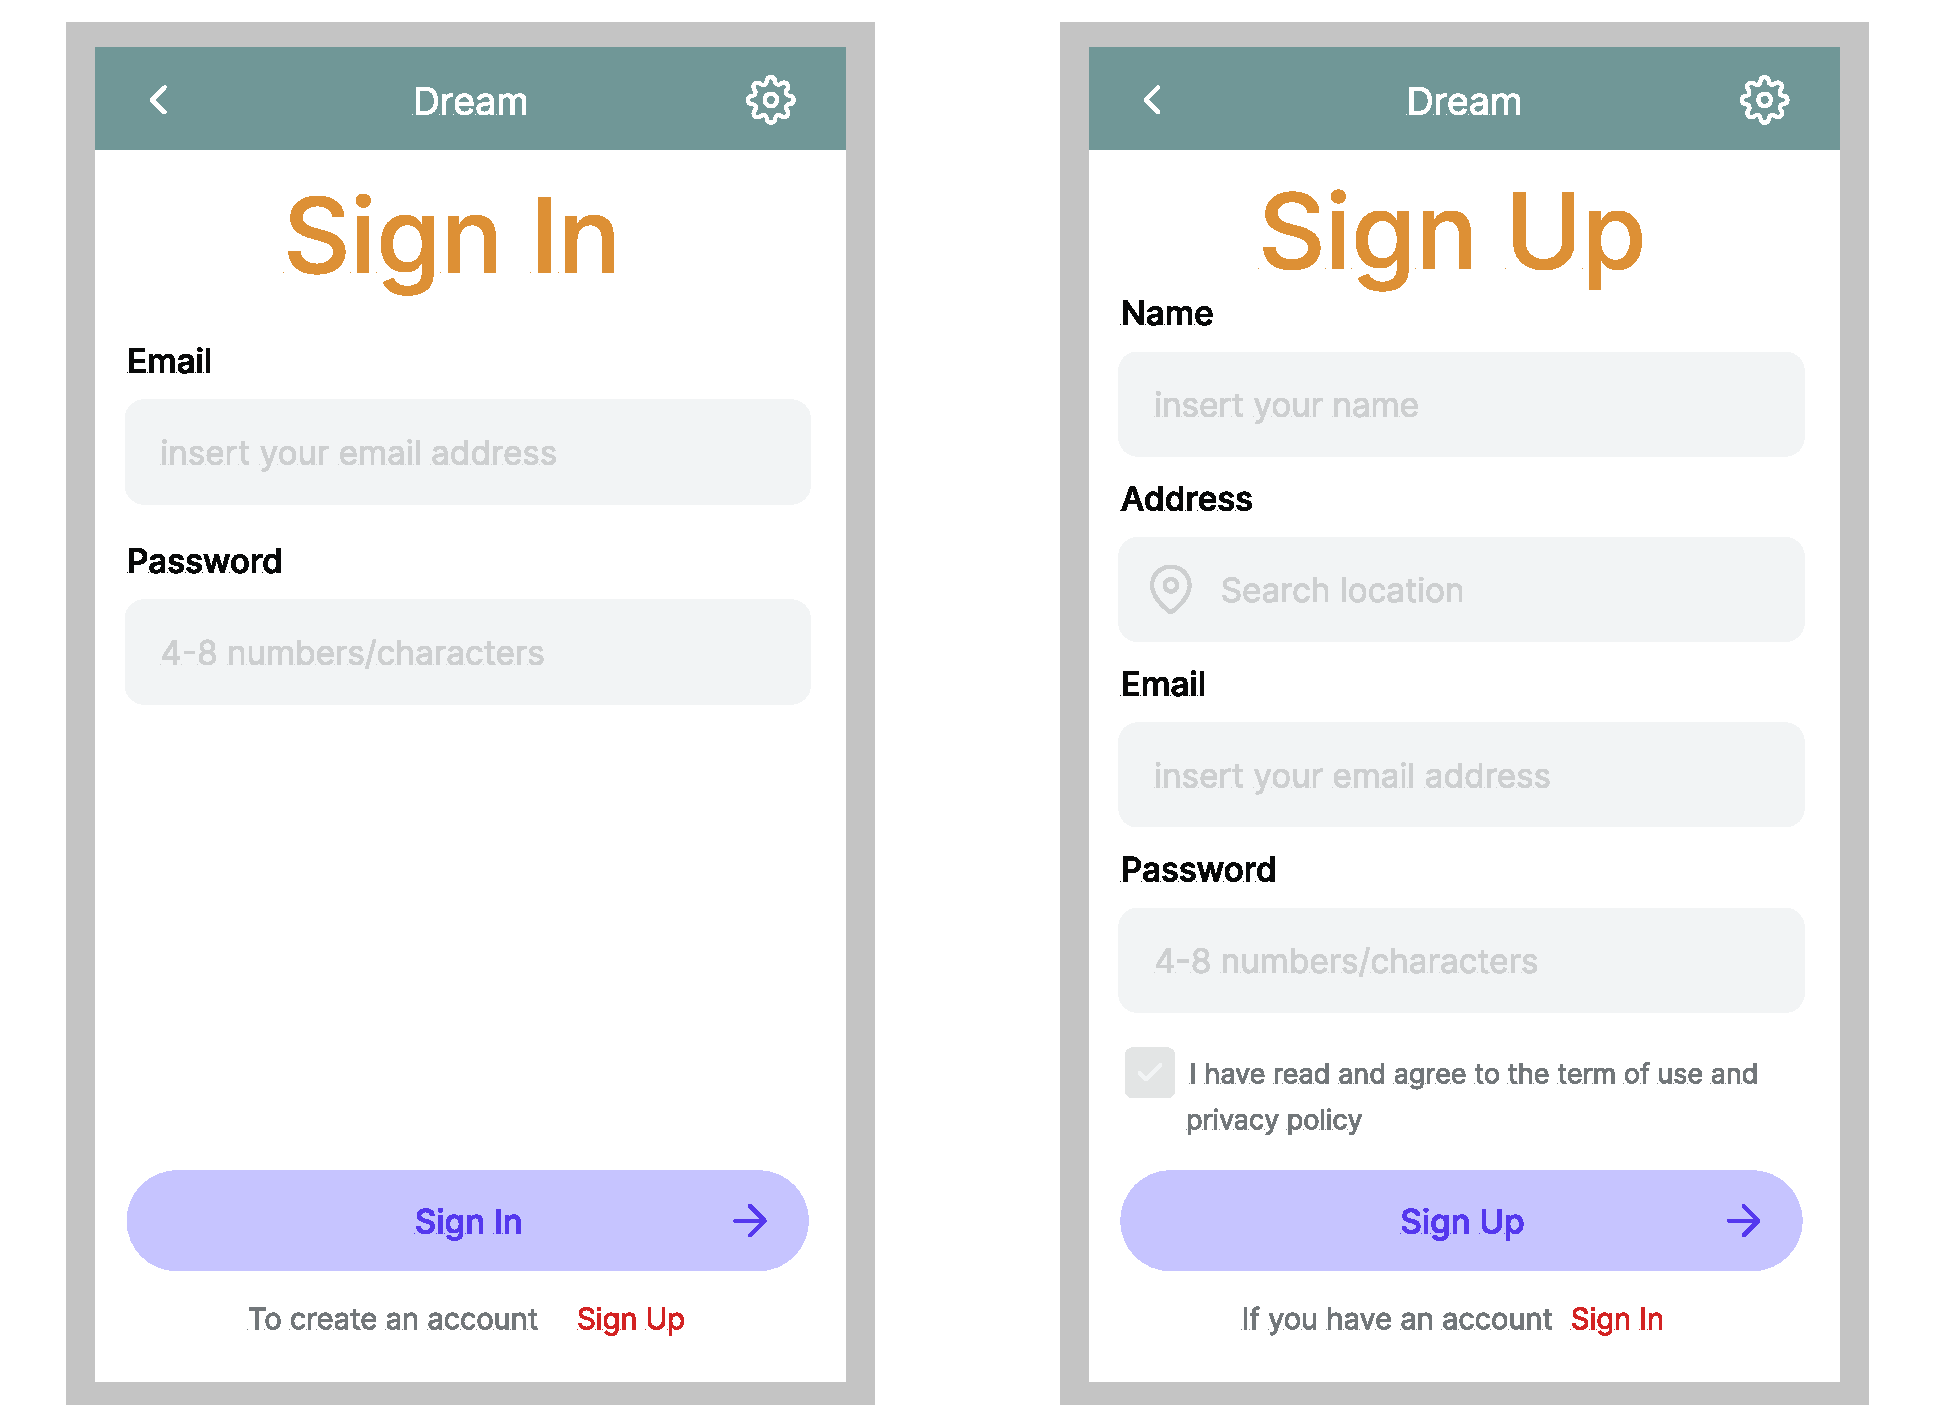
\includegraphics[page=1, width=\textwidth]{Images/sign_up_in.JPG}
<<<<<<< HEAD
	\caption{\label{fig:FE_image1}Sign Up, Sign In}
=======
	\caption{\label{fig:FE_image}Sign Up, Sign In}
>>>>>>> bea6cd44afb95a3d236ec690d06eb9849ecd2ae9
\end{figure}

\begin{figure}[H]
	\centering
    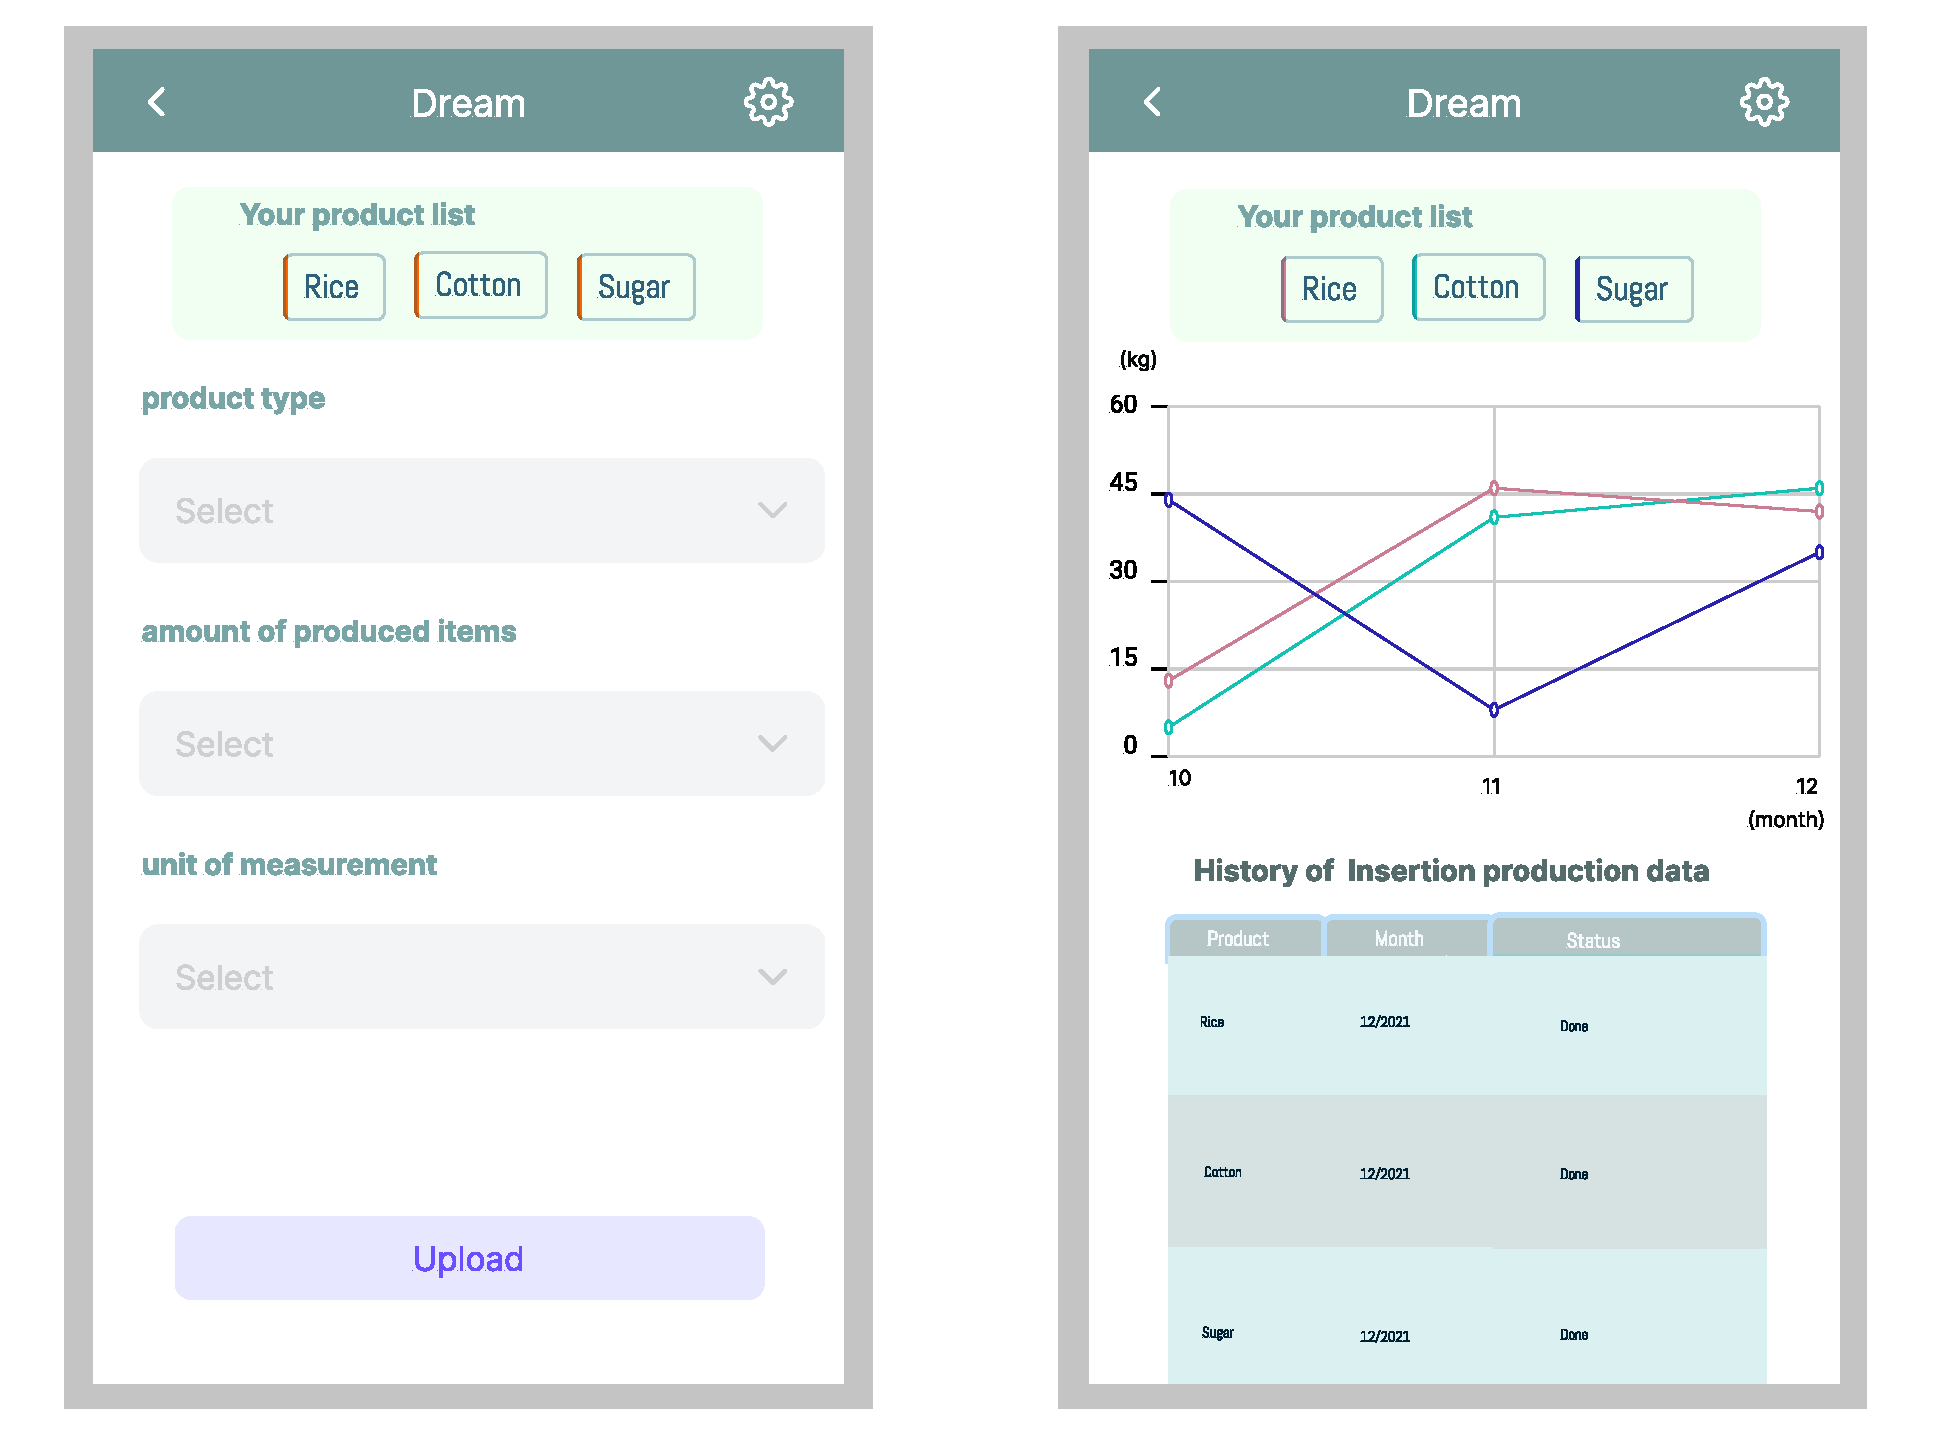
\includegraphics[page=1, width=\textwidth]{Images/product_amount_registration.JPG}
<<<<<<< HEAD
	\caption{\label{fig:FE_image2}Product registration, Amount registration}
=======
	\caption{\label{fig:FE_image}Product registration, Amount registration}
>>>>>>> bea6cd44afb95a3d236ec690d06eb9849ecd2ae9
\end{figure}



\begin{figure}[H]
	\centering
    \includegraphics[page=1, width=\textwidth]{Images/message_insertion.JPG}
<<<<<<< HEAD
	\caption{\label{fig:FE_image3}Message insertion}
=======
	\caption{\label{fig:FE_image}Message insertion}
>>>>>>> bea6cd44afb95a3d236ec690d06eb9849ecd2ae9
\end{figure}

\begin{figure}[H]
	\centering
    \includegraphics[page=1, width=\textwidth]{Images/desktop_chat.JPG}
<<<<<<< HEAD
	\caption{\label{fig:FE_image4}Desktop chat}
=======
	\caption{\label{fig:FE_image}Desktop chat}
>>>>>>> bea6cd44afb95a3d236ec690d06eb9849ecd2ae9
\end{figure}
\subsubsection{Hardware Interfaces}

\subsubsection{Software Interfaces}

\subsubsection{Communication Interfaces}


\subsection{Functional Requirements}
In this section we present the main \textbf{functional requirements} of the application while organizing them based on the actor that 

% #################### USE CASES TABLES ####################
\subsubsection{Users}
\label{sect:users_requirements}
% USE CASE TABLE 1: SIGN UP
 In this section there will be presented users use case tables \ldots
\begin{table}[H]
    \centering
    \begin{tabular}[c]{|l|p{0.75\textwidth}|}
        \hline % ---------------------------------------------------------------------
    	\textsc{id}                 &   1\\
    	\hline % ---------------------------------------------------------------------
    	\textsc{Name}               &   Sign up User with email\\
    	\hline % ---------------------------------------------------------------------
    	\textsc{Actors}             &   User\\
    	\hline % ---------------------------------------------------------------------
    	\textsc{Entry conditions}   &   User has opened the Web page OR User has downloaded and opened the application on his smartphone\\
    	\hline % ---------------------------------------------------------------------
    	\textsc{Input}   &   Email to use for the registration\\
    	\hline % ---------------------------------------------------------------------
    	\textsc{Event flow}         &   %\footnotesize
            	                        \begin{itemize}
                                    	    \item The system displays the “Sign in” page
                                            \item User clicks on “Sign up”
                                            \item The system displays two fields: email and password
                                            \item User inserts the data and accepts the “Terms of services”
                                            \item User clicks on the “Confirm” button
                                            \item The system displays the acceptance of the registration and invites User to go to his inbox in order to confirm the registration
                                            \item User opens his inbox, checks the email and clicks on the confirmation link

                                        \end{itemize}\\
        \hline % ---------------------------------------------------------------------
        \textsc{Exit conditions}    &  User registration has been successful: user data are stored in the system’s database. User can now login with his credentials\\
    	\hline % ---------------------------------------------------------------------
    	\textsc{Output}             &  \begin{itemize}
    	    \item User’s email is stored in the system’s database
            \item User receives the confirmation email

    	\end{itemize}\\
    	\hline % ---------------------------------------------------------------------
    	\textsc{Exceptions}         &  \begin{itemize}
    	    \item User inserts an email which is already stored in the database. So, after User clicks on “Confirm”, the system displays an error page which tells that User is already registered to the service and invites him to login with that email
            \item User inserts an invalid email. So, after User clicks on “Confirm”, the system displays the same sign up page with an error message, which suggests User to check the inserted email or to change it

    	\end{itemize}\\
    	\hline % ---------------------------------------------------------------------
        
    \end{tabular}
    \caption{\label{tab:user_sign_up}User caption \textnumero 1}
\end{table}

\begin{table}[H]
    \centering
    \begin{tabular}[c]{|l|p{0.75\textwidth}|}
        \hline % ---------------------------------------------------------------------
    	\textsc{id}                 &   2\\
    	\hline % ---------------------------------------------------------------------
    	\textsc{Name}               &   Login User\\
    	\hline % ---------------------------------------------------------------------
    	\textsc{Actors}             &   User\\
    	\hline % ---------------------------------------------------------------------
    	\textsc{Entry conditions}   &   User has opened the Web page OR User has downloaded and opened the application on his smartphone\\
    	\hline % ---------------------------------------------------------------------
    	\textsc{Input}   &   User’s valid email and password\\
    	\hline % ---------------------------------------------------------------------
    	\textsc{Event flow}         &   %\footnotesize
            	                        \begin{itemize}
                                    	    \item The system displays the “Login” page
                                            \item User inserts his credentials (email, password) and clicks the “Login” button
                                            \item The system checks the correctness of the inserted credentials
                                            \item The system displays the home page


                                        \end{itemize}\\
        \hline % ---------------------------------------------------------------------
        \textsc{Exit conditions}    &  User is logged in\\
    	\hline % ---------------------------------------------------------------------
    	\textsc{Output}             &  \begin{itemize}
    	    \item User inserts a wrong combination of email and password. The system displays the same page with an error message.

    	\end{itemize}\\
    	\hline % ---------------------------------------------------------------------
    	\textsc{Exceptions}         &  \begin{itemize}
    	    \item User inserts an email which is already stored in the database. So, after User clicks on “Confirm”, the system displays an error page which tells that User is already registered to the service and invites him to login with that email
            \item User inserts an invalid email. So, after User clicks on “Confirm”, the system displays the same sign up page with an error message, which suggests User to check the inserted email or to change it

    	\end{itemize}\\
    	\hline % ---------------------------------------------------------------------
        
    \end{tabular}
    \caption{\label{tab:user_login}User caption \textnumero 2}
\end{table}

\subsubsection{Policy makers}
\textbf{\textcolor{myblue}{Use case diagram}}
\begin{figure}[H]
	\centering
    \includegraphics[page=1, width=\textwidth]{Images/ud_policy.JPG}
	\caption{\label{fig:use_case_diagram}Policy maker's use case diagram}
\end{figure}
\label{sect:policy_maker_requirements}
% Moved to section 1.4 Definitions, acronyms, abbreviations


\begin{table}[H]
    \centering
    \begin{tabular}{|l|p{0.75\textwidth}|}
        \hline % ---------------------------------------------------------------------
    	\textsc{id}                 &   1\\
    	\hline % ---------------------------------------------------------------------
    	\textsc{Name}               &   Visualize the performance data of each farmer\\
    	\hline % ---------------------------------------------------------------------
    	\textsc{Actors}             &   Policy maker\\
    	\hline % ---------------------------------------------------------------------
    	\textsc{Entry conditions}   &   Policy maker has logged in\\
    	\hline % ---------------------------------------------------------------------
    	\textsc{Event flow}         &   %\footnotesize
            	                        \begin{itemize}
                                    	    \item Policy maker presses the button “Farmer’s performance”
                                    		\item The system displays a page with list of farmer divided by performances
                                    		\item Policy maker selects interested farmer’s name
                                    		\item The system shows the detailed information about farmer’s production
                                        \end{itemize}\\
        \hline % ---------------------------------------------------------------------
        \textsc{Exit conditions}    &  The system returns to the main page of policy maker\\
    	\hline % ---------------------------------------------------------------------
    	\textsc{Output}             &  \begin{itemize}
    	    \item Policy maker has obtained the data they were looking for
    	\end{itemize}\\
    	\hline % ---------------------------------------------------------------------
    	\textsc{Exceptions}         &  Policy maker couldn’t find the name of farmer who should exist\\
    	\hline % ---------------------------------------------------------------------
        
    \end{tabular}
    \caption{\label{tab:visualize_farmer_performance}Use case table that describes one of the policy maker functional requirements:  the capability of visualizing the farmer's information categorized by their performance} %TODO: add caption
\end{table}

\begin{figure}[H]
    \centering
    \includegraphics[scale=0.5]{Images/Sequence diagrams/PolicyMaker - visualize performance.pdf}
    \caption{Caption}
    \label{fig:my_label}
\end{figure}

\begin{table}[H]
    \centering
    \begin{tabular}{|l|p{0.75\textwidth}|}
        \hline % ---------------------------------------------------------------------
    	\textsc{id}                 &   2\\
    	\hline % ---------------------------------------------------------------------
    	\textsc{Name}               &   Visualize the incentive status data\\
    	\hline % ---------------------------------------------------------------------
    	\textsc{Actors}             &   Policy maker\\
    	\hline % ---------------------------------------------------------------------
    	\textsc{Entry conditions}   &   Policy maker has logged in\\
    	\hline % ---------------------------------------------------------------------
    	\textsc{Event flow}         &   %\footnotesize
            	                        \begin{itemize}
                                    	    \item Policy maker presses the button “Farmer’s performance”
                                    		\item The system displays a page with list of farmer divided by performance, at the place of high performer there will be a column which clarifies the status of incentive 
                                       		\item Policy maker selects interested farmer’s incentive column
                                    		\item The system shows the detailed information about farmer’s incentive status
                                        \end{itemize}\\
        \hline % ---------------------------------------------------------------------
        \textsc{Exit conditions}    &  The system returns to the main page of policy maker\\
    	\hline % ---------------------------------------------------------------------
    	\textsc{Output}             &  \begin{itemize}
    	    \item Policy maker has obtained the data they were looking for
    	\end{itemize}\\
    	\hline % ---------------------------------------------------------------------
    	\textsc{Exceptions}         &  Policy maker couldn’t find the name of farmer who should exist\\
    	\hline % ---------------------------------------------------------------------
        
    \end{tabular}
    \caption{\label{tab:visualize_incentives}Use case table that describes one of the policy maker functional requirements:  the capability of tracking the incentive statuses} %TODO: add caption
\end{table}

\begin{figure}[H]
    \centering
    \includegraphics[scale=0.5]{Images/Sequence diagrams/PolicyMaker - visualise incentive status.pdf}
    \caption{Caption}
    \label{fig:my_label}
\end{figure}

\begin{table}[H]
    \centering
    \begin{tabular}{|l|p{0.75\textwidth}|}
        \hline % ---------------------------------------------------------------------
    	\textsc{id}                 &   3\\
    	\hline % ---------------------------------------------------------------------
    	\textsc{Name}               &   Visualize the correlation of history of visiting and improvement of farmer's performance\\
    	\hline % ---------------------------------------------------------------------
    	\textsc{Actors}             &   Policy maker\\
    	\hline % ---------------------------------------------------------------------
    	\textsc{Entry conditions}   &   Policy maker has logged in\\
    	\hline % ---------------------------------------------------------------------
    	\textsc{Event flow}         &   %\footnotesize
            	                        \begin{itemize}
                                    	    \item Policy maker presses the button “Performance transition”
                                    		\item The system displays a page with categorized farmer, also it highlights the farmers who have improved their performance significantly within a year
                                    		\item Policy maker selects interested farmer’s name
                                    		\item The system shows the detailed information about farmer’s monthly performance transition 
                                        \end{itemize}\\
        \hline % ---------------------------------------------------------------------
        \textsc{Exit conditions}    &  The system returns to the main page of policy maker\\
    	\hline % ---------------------------------------------------------------------
    	\textsc{Output}             &  \begin{itemize}
    	    \item Policy maker has obtained the data they were looking for
    	\end{itemize}\\
    	\hline % ---------------------------------------------------------------------
    	\textsc{Exceptions}         &  Policy maker couldn’t find the name of farmer who should exist\\
    	\hline % ---------------------------------------------------------------------
        
    \end{tabular}
    \caption{\label{tab:visualize_iprovement}Use case table that describes one of the policy maker functional requirements:  the capability of tracking the transition of farmer's performance due to the visits of agronomists} %TODO: add caption
\end{table}

\begin{figure}[H]
    \centering
    \includegraphics[scale=0.5]{Images/Sequence diagrams/PolicyMaker - visualise correlation and improvement.pdf}
    \caption{Caption}
    \label{fig:my_label}
\end{figure}


\subsubsection{Farmers}
\textbf{\textcolor{myblue}{Use case diagram}}
\begin{figure}[H]
	\centering
    \includegraphics[page=1, width=\textwidth]{Images/ud_fa.JPG}
	\caption{\label{fig:use_case_diagram}Farmer's use case diagram}
\end{figure}
\label{sect:farmer_requirements}
Synonims: system, application, service



% ####################### 1 PRODUCTION DATA UPLOAD ###################

\begin{table}[H]
    \centering
    \begin{tabular}[c]{|l|p{0.75\textwidth}|}
        \hline % ---------------------------------------------------------------------
    	\textsc{id}                 &   1\\
    	\hline % ---------------------------------------------------------------------
    	\textsc{Name}               &   Production data upload\\
    	\hline % ---------------------------------------------------------------------
    	\textsc{Actors}             &   Farmer\\
    	\hline % ---------------------------------------------------------------------
    	\textsc{Entry conditions}   &   Farmer has logged in\\
    	\hline % ---------------------------------------------------------------------
    	\textsc{Event flow}         &   %\footnotesize
            	                        \begin{itemize}
                                    	    \item Farmer selects the graphical element for recording production data, called informally \textit{Record Production Data button} for the sake of simplicity
                                    		\item The application displays a section that asks for more information (mandatory fields like type of production, amount of produced items, unit of measurement and optional one like description of the productivity, notes) and an element to save and upload informations, called informally \textit{Upload Button}
                                    		\item Farmer fills the mandatory fields of the current section and eventually the optional ones. Then press the Upload Button.
                                    		\item The application displays a confirm popup revealing the summary of the information is going to be recorded, asking for Farmer confirmation through a \textit{Confirm Button}
                                    		\item The farmer confirms the submission by selecting the Confirm Button
                                        \end{itemize}\\
        \hline % ---------------------------------------------------------------------
        \textsc{Exit conditions}    &  The application displays the summary page of both already uploaded product information and the previous submitted ones\\
    	\hline % ---------------------------------------------------------------------
    	\textsc{Output}             &  \begin{itemize}
    	    \item The system collects the new production data
    	    \item The farmer can visualize the list of both current production information and the previous ones
    	   % TODO (where can he visualize it?)
    	\end{itemize}\\
    	\hline % ---------------------------------------------------------------------
    	\textsc{Exceptions}         &  Farmer submits production data without filling the mandatory fields. In such case, the system displays an error message informing the Farmer about the missing field(s) required in order to achieve the goal\\
    	\hline % ---------------------------------------------------------------------
        
    \end{tabular}
    \caption{\label{tab:Production_data_submission}Use case table that describes one of the farmer functional requirements: the capability of submitting in the system his activity's usual production information.}
\end{table}


\begin{figure}[H]
	\centering
    \includegraphics[page=1, width=\textwidth]{Images/SeqDiag/product_info_upload_seq_diag.pdf}
	\caption{\label{fig:product_info_seq_diag}High level UML sequence diagram of the production data submission process}
\end{figure}


% ####################### 2 SUGGESTION REQUEST ###################

\begin{table}[H]
    \centering
    \begin{tabular}{|l|p{0.75\textwidth}|}
        \hline % ---------------------------------------------------------------------
    	\textsc{id}                 &   2\\
    	\hline % ---------------------------------------------------------------------
    	\textsc{Name}               &   Help/suggestion request\\
    	\hline % ---------------------------------------------------------------------
    	\textsc{Actors}             &   Farmer\\
    	\hline % ---------------------------------------------------------------------
    	\textsc{Entry conditions}   &   Farmer has logged in\\
    	\hline % ---------------------------------------------------------------------
    	\textsc{Event flow}         &   %\footnotesize
            	                        \begin{itemize}
                                    	    \item Farmer selects the graphical section responsible of the private requests, called informally \textit{request section} for the sake of simplicity
                                    		\item The application displays a section that presents an eventual list of previous request chats, and an internal element to send a new private request, called informally \textit{Send request element}
                                    		\item Farmer selects the send request button
                                    		\item The application displays a new section that present all the Farmer's saved contacts
                                    		\item The farmer selects the contact he wants to send the request
                                    		\item The system displays a section with an editable text form and a send button.
                                    		\item The farmer writes the request and selects the send button
                                        \end{itemize}\\
        \hline % ---------------------------------------------------------------------
        \textsc{Exit conditions}    &  The application displays the summary page of both already sent request chat and the previous submitted ones\\
    	\hline % ---------------------------------------------------------------------
    	\textsc{Output}             &  \begin{itemize}
    	    \item The system collects the new request chat
    	    \item The farmer can visualize the list of both current request chat and the previous ones
    	   % TODO (where can he visualize it?)
    	\end{itemize}\\
    	\hline % ---------------------------------------------------------------------
    	\textsc{Exceptions}         &  Farmer selects the request button without editing the text form. In such case, the system displays an error message informing the Farmer about the missing field required in order to achieve the goal\\
    	\hline % ---------------------------------------------------------------------
        
    \end{tabular}
    \caption{\label{tab:Help_request_submission}Use case table that describes one of the farmer functional requirements: the capability of submitting in the system help requests to other farmers and/or agronomists in a private way.}

\end{table}

\begin{figure}[H]
	\centering
    \includegraphics[page=1, width=\textwidth]{Images/SeqDiag/help_request_seq_diag.pdf}
	\caption{\label{fig:help_request_seq_diag}High level UML sequence diagram of the help request process}
\end{figure}

% ####################### 3 FORUM GENERATION ###################

\begin{table}[H]
    \centering
    \begin{tabular}{|l|p{0.75\textwidth}|}
        \hline % ---------------------------------------------------------------------
    	\textsc{id}                 &   3\\
    	\hline % ---------------------------------------------------------------------
    	\textsc{Name}               &   Forum generation\\
    	\hline % ---------------------------------------------------------------------
    	\textsc{Actors}             &   Farmer\\
    	\hline % ---------------------------------------------------------------------
    	\textsc{Entry conditions}   &   Farmer has logged in\\
    	\hline % ---------------------------------------------------------------------
    	\textsc{Event flow}         &   %\footnotesize
            	                        \begin{itemize}
                                    	    \item Farmer selects the graphical section responsible of the forum generation, called informally \textit{Forum section} for the sake of simplicity
                                    		\item The application displays a section that presents an eventual list that contains both previous submitted forums and farmer's forum replies, and an internal element to submit a new public forum, called informally \textit{forum upload button}
                                    		\item Farmer selects the forum upload button
                                    		\item The application displays a new section that present 3 mandatory fields (the topic/context of the thread, the title and the question content) and a submission button
                                    		\item The farmer fills all the mandatory fields and selects the submission button
                                    		\item The application displays a confirm popup revealing the summary of the information is going to be uploaded, asking for Farmer confirmation through a \textit{Confirm Button}
                                    		\item The farmer confirms the submission by selecting the Confirm Button
                                        \end{itemize}\\
        \hline % ---------------------------------------------------------------------
        \textsc{Exit conditions}    &  The application displays the summary page containing both already submitted forum thread, the previous submitted ones and the ones whose the farmer replied\\
    	\hline % ---------------------------------------------------------------------
    	\textsc{Output}             &  \begin{itemize}
    	    \item The system collects the new forum thread
    	    \item The farmer can visualize the list containing both current forum thread, the previous submitted ones and the ones whose the farmer replied
    	   % TODO (where can he visualize it?)
    	\end{itemize}\\
    	\hline % ---------------------------------------------------------------------
    	\textsc{Exceptions}         &   Farmer submits Forum thread without filling all the mandatory fields. In such case, the system displays an error message informing the Farmer about the missing field(s) required in order to achieve the goal\\
    	\hline % ---------------------------------------------------------------------
        
    \end{tabular}

\caption{\label{tab:Forum_generation}Use case table that describes one of the farmer functional requirements: the capability of submitting in the system public forum threads}
\end{table}

\begin{figure}[H]
	\centering
    \includegraphics[page=1, width=\textwidth]{Images/SeqDiag/forum_generation_seq_diag.pdf}
	\caption{\label{fig:forum_generation_seq_diag}High level UML sequence diagram of the forum generation process}
\end{figure}

% ####################### 4 PROBLEM INFORMATION ###################

\begin{table}[H]
    \centering
    \begin{tabular}{|l|p{0.75\textwidth}|}
        \hline % ---------------------------------------------------------------------
    	\textsc{id}                 &   4\\
    	\hline % ---------------------------------------------------------------------
    	\textsc{Name}               &   Problem information upload\\
    	\hline % ---------------------------------------------------------------------
    	\textsc{Actors}             &   Farmer\\
    	\hline % ---------------------------------------------------------------------
    	\textsc{Entry conditions}   &   Farmer has logged in\\
    	\hline % ---------------------------------------------------------------------
    	\textsc{Event flow}         &   %\footnotesize
            	                        \begin{itemize}
                                    	    \item Farmer selects the graphical section responsible for the problem information submission, called informally \textit{Problems section}
                                    		\item The application displays a section that requires for information (described previously) and a "submit button"
                                    		\item Farmer fills the mandatory fields and eventually the optional ones, then selects the upload button
                                    		\item The application displays a confirm popup revealing the summary of the information is going to be uploaded, asking for Farmer confirmation through a \textit{Confirm Button}
                                    		\item The farmer confirms the submission by selecting the Confirm Button
                                        \end{itemize}\\
        \hline % ---------------------------------------------------------------------
        \textsc{Exit conditions}    &  The application displays the summary page containing both already submitted problem information and the previous submitted ones\\
    	\hline % ---------------------------------------------------------------------
    	\textsc{Output}             &  \begin{itemize}
    	    \item The system collects the new problem information instance
    	    \item The farmer can visualize the list containing both the current submitted problem information and the previous submitted ones
    	   % TODO (where can he visualize it?)
    	\end{itemize}\\
    	\hline % ---------------------------------------------------------------------
    	\textsc{Exceptions}         &   Farmer submits problem information without filling all the mandatory fields. In such case, the system displays an error message informing the Farmer about the missing field(s) required in order to achieve the goal\\
    	\hline % ---------------------------------------------------------------------
        
    \end{tabular}

\caption{\label{tab:problem_information}Use case table that describes one of the farmer functional requirements: the capability of submitting in the system problem information}
\end{table}

% ####################### 5 GOOD PRACTICES ###################

\begin{table}[H]
    \centering
    \begin{tabular}{|l|p{0.75\textwidth}|}
        \hline % ---------------------------------------------------------------------
    	\textsc{id}                 &   5\\
    	\hline % ---------------------------------------------------------------------
    	\textsc{Name}               &   Good practices upload\\
    	\hline % ---------------------------------------------------------------------
    	\textsc{Actors}             &   Farmer\\
    	\hline % ---------------------------------------------------------------------
    	\textsc{Entry conditions}   &   Farmer has logged in\\
    	\hline % ---------------------------------------------------------------------
    	\textsc{Event flow}         &   %\footnotesize
            	                        \begin{itemize}
                                    	    \item Farmer selects the graphical section responsible for the good practices document submission, called informally \textit{document section}
                                    		\item The application displays a section that requires for information (described previously) and a "submit button"
                                    		\item Farmer fills the mandatory fields and eventually the optional ones, then selects the upload button
                                    		\item The farmer confirms the submission by selecting the Confirm Button
                                        \end{itemize}\\
        \hline % ---------------------------------------------------------------------
        \textsc{Exit conditions}    &  The application displays the summary page containing both already submitted document and the previous submitted ones\\
    	\hline % ---------------------------------------------------------------------
    	\textsc{Output}             &  \begin{itemize}
    	    \item The system collects the new document
    	    \item The farmer can visualize the list containing both the current submitted document and the previous submitted ones
    	   % TODO (where can he visualize it?)
    	\end{itemize}\\
    	\hline % ---------------------------------------------------------------------
    	\textsc{Exceptions}         &   Farmer submits document without filling all the mandatory fields. In such case, the system displays an error message informing the Farmer about the missing field(s) required in order to achieve the goal\\
    	\hline % ---------------------------------------------------------------------
        
    \end{tabular}

\caption{\label{tab:good_practice_submission}Use case table that describes one of the farmer functional requirements: the capability of submitting in the system good practices document}
\end{table}

\begin{figure}[H]
	\centering
    \includegraphics[page=1, width=\textwidth]{Images/SeqDiag/good_practice_seq_diag.pdf}
	\caption{\label{fig:good_practice_seq_diag}High level UML sequence diagram of the good practices document submission process}
\end{figure}


\begin{table}[H]
    \centering
    \begin{tabular}{|l|p{0.75\textwidth}|}
        \hline % ---------------------------------------------------------------------
    	\textsc{id}                 &   6\\
    	\hline % ---------------------------------------------------------------------
    	\textsc{Name}               &   Visualize relevant data\\
    	\hline % ---------------------------------------------------------------------
    	\textsc{Actors}             &   Farmer\\
    	\hline % ---------------------------------------------------------------------
    	\textsc{Entry conditions}   &   Farmer has logged in\\
    	\hline % ---------------------------------------------------------------------
    	\textsc{Event flow}         &   %\footnotesize
            	                        \begin{itemize}
                                    	    \item Farmer selects the graphical section responsible for the relevant data visualization, called informally \textit{Relevant section}
                                        \end{itemize}\\
        \hline % ---------------------------------------------------------------------
        \textsc{Exit conditions}    &  The application displays a section containing information about weather forecasts, farm related tools suggestion, agronomist visit time, amount of water used that month, soil humidity etc.)\\
    	\hline % ---------------------------------------------------------------------
    	\textsc{Output}             &  \begin{itemize}
    	    \item The farmer can visualize relevant informations
    	    \item Farmer can interact with information (links to shop websites etc.)
    	   % TODO (where can he visualize it?)
    	\end{itemize}\\
    	\hline % ---------------------------------------------------------------------
    	\textsc{Exceptions}         &   If the internet connection is lost, the application displays a section informing the task cannot be achieved\\
    	\hline % ---------------------------------------------------------------------
        
    \end{tabular}

\caption{\label{tab:visualize_relevant_data}Use case table that describes one of the farmer goals: visualize relevant data}
\end{table}

\subsubsection{Agronomists}
\textbf{\textcolor{myblue}{Use case diagram}}
\begin{figure}[H]
	\centering
    \includegraphics[page=1, width=\textwidth]{Images/ud_ag.JPG}
	\caption{\label{fig:use_case_diagram}Agronomist's use case diagram}
\end{figure}
\label{sect:agronomist_requirements}
% USE CASE TABLE 1: INSERT THE AREA AGRONOMISTS ARE RESPONSIBLE OF
 In this section there will be presented agronomists use case tables \ldots
\begin{table}[H]
    \centering
    \begin{tabular}[c]{|l|p{0.75\textwidth}|}
        \hline % ---------------------------------------------------------------------
    	\textsc{id}                 &   1\\
    	\hline % ---------------------------------------------------------------------
    	\textsc{Name}               &   Insert the area they are responsible of\\
    	\hline % ---------------------------------------------------------------------
    	\textsc{Actors}             &   Agronomist\\
    	\hline % ---------------------------------------------------------------------
    	\textsc{Entry conditions}   &   Agronomist has logged in\\
    	\hline % ---------------------------------------------------------------------
    	\textsc{Event flow}         &   \footnotesize
            	                        \begin{itemize}
                                    	    \item Agronomist presses the button “insert the area”
                                    		\item The system displays a page with all the available areas and a search bar
                                    		\item (Agronomist makes a research based on the name/location of the area)
                                    		\item (The system shows the results)
                                    		\item Agronomist selects the desired area
                                    		\item The system shows the details of the area selected
                                    		\item Agronomist clicks on “Insert this area”
                                    		\item The system updates the database and shows a message of insertion completed
                                        \end{itemize}\\
        \hline % ---------------------------------------------------------------------
        \textsc{Exit conditions}    &  The system returns to the main home\\
    	\hline % ---------------------------------------------------------------------
    	\textsc{Output}             &  \begin{itemize}
    	    \item The system has added the agronomist in the database as responsible for that area
    	\end{itemize}\\
    	\hline % ---------------------------------------------------------------------
    	\textsc{Exceptions}         &  \begin{itemize}
    	    \item Agronomist wrongly clicks “Insert this area”. The system displays a popup notifying that he will be added as responsible for that area and the agronomist clicks on “Cancel” button
    	    \item (caso 1 agronomist 1 area) Agronomist chooses an area which already has a responsible agronomist. The system displays an error message.
    	\end{itemize}\\
    	\hline % ---------------------------------------------------------------------
        
    \end{tabular}
    \caption{\label{tab:responsible_area_insertion}Agronomist caption \textnumero 1}
\end{table}

\includegraphics[scale=0.5]{Images/Sequence diagrams/Agronomist - Insert area.png}

% USE CASE TABLE 2: ACCESS THE "REQUEST FOR HELP" SECTION

\begin{table}[H]
    \centering
    \begin{tabular}[c]{|l|p{0.75\textwidth}|}
        \hline % ---------------------------------------------------------------------
    	\textsc{id}                 &   2\\
    	\hline % ---------------------------------------------------------------------
    	\textsc{Name}               &   Visualise and answer to requests for help\\
    	\hline % ---------------------------------------------------------------------
    	\textsc{Actors}             &   Agronomist\\
    	\hline % ---------------------------------------------------------------------
    	\textsc{Entry conditions}   &   Agronomist has logged in\\
    	\hline % ---------------------------------------------------------------------
    	\textsc{Event flow}         &   \footnotesize
            	                        \begin{itemize}
                                    	    \item Agronomist goes to the “Requests for help” section
                                    		\item The system extracts the data from the database and displays a search bar and the list of conversations (sorted by recent activity), marking the ones which contains new messages
                                    		\item Agronomist selects a conversation
                                    		\item The system displays all the messages contained in that conversation and a text box
                                    		\item Agronomist writes in the text box an answer to the request and clicks “Send”
                                    		\item The system adds the message to the database
                                        \end{itemize}\\
        \hline % ---------------------------------------------------------------------
        \textsc{Exit conditions}    &  The system remains in the same page, refreshing its content\\
    	\hline % ---------------------------------------------------------------------
    	\textsc{Output}             &  \begin{itemize}
    	    \item The system adds the message to the database
    	    \item The system notifies the participants of that conversation about the new message
    	\end{itemize}\\
    	\hline % ---------------------------------------------------------------------
    	\textsc{Exceptions}         &  The system cannot connect to the database/server. The system displays an error message.\\
    	\hline % ---------------------------------------------------------------------
        
    \end{tabular}
    \caption{\label{tab:help_request_section_access}Agronomist caption \textnumero 2}
\end{table}

\includegraphics[scale=0.5]{Images/Sequence diagrams/Agronomist - Visualise and answer to requests for help.png}

% USE CASE TABLE 3: VISUALIZE DATA OF THE AREA

\begin{table}[H]
    \centering
    \begin{tabular}[c]{|l|p{0.75\textwidth}|}
        \hline % ---------------------------------------------------------------------
    	\textsc{id}                 &   3\\
    	\hline % ---------------------------------------------------------------------
    	\textsc{Name}               &   Visualize data of the area (weather forecasts, best/under performing farmers)\\
    	\hline % ---------------------------------------------------------------------
    	\textsc{Actors}             &   Agronomist\\
    	\hline % ---------------------------------------------------------------------
    	\textsc{Entry conditions}   &   Agronomist has logged in\\
    	\hline % ---------------------------------------------------------------------
    	\textsc{Event flow}         &   \footnotesize
            	                        \begin{itemize}
                                    	    \item Agronomist goes to the “Information about the area” section
                                    		\item The system displays a page with two main options: “Weather forecasts” and “Farmers’ performing situation”
                                    		\item Agronomist selects  the “Weather forecasts” section
                                    		\item The system extracts the data from the database and shows all the information concerning the weather forecasts in that area (...)
                                    		\item Agronomist selects the “Farmers’ performing situation” section
                                    		\item The system extracts the data from the database and displays the list of all the farmers in the area, grouping them in “Best performing”, “Normal performing” and “Under-performing”
                                        \end{itemize}\\
        \hline % ---------------------------------------------------------------------
        \textsc{Exit conditions}    &  The system returns to the main page (?)\\
    	\hline % ---------------------------------------------------------------------
    	\textsc{Output}             &  \begin{itemize}
    	    \item %TODO
    	\end{itemize}\\
    	\hline % ---------------------------------------------------------------------
    	\textsc{Exceptions}         &  %TODO
    	\\
    	\hline % ---------------------------------------------------------------------
        
    \end{tabular}
    \caption{\label{tab:Area_information_access}Agronomist caption \textnumero 3}
\end{table}

\includegraphics[scale=0.5]{Images/Sequence diagrams/Agronomist - Visualise data of the area.png}

% USE CASE TABLE 4: ACCESS THE "DAILY PLAN" SECTION


\begin{table}[H]
    \centering
    \begin{tabular}[c]{|l|p{0.75\textwidth}|}
        \hline % ---------------------------------------------------------------------
    	\textsc{id}                 &   4\\
    	\hline % ---------------------------------------------------------------------
    	\textsc{Name}               &   Visualise and update a daily plan\\
    	\hline % ---------------------------------------------------------------------
    	\textsc{Actors}             &   Agronomist\\
    	\hline % ---------------------------------------------------------------------
    	\textsc{Entry conditions}   &   \begin{itemize}
                                    	    \item Agronomist has logged in
                                    	    \item At least one daily plan is present
                                        \end{itemize}\\
    	\hline % ---------------------------------------------------------------------
    	\textsc{Event flow}         &   \footnotesize
            	                        \begin{itemize}
                                    	    \item Agronomist goes to the “Daily Plan” section, which is divided in “Visualise/Update” and “Confirm/Specify deviation from”. Agronomist selects the “Visualise/Update” section
                                    		\item The system extracts the data from the database and displays the list of daily plans for that agronomist
                                    		\item Agronomist selects a daily plan
                                    		\item The system displays all the information about that daily plan (day-month-year, farmers to be visited)
                                    		\item Agronomist clicks on the “Update” button
                                    		\item The system displays the list of farmers contained in the selected daily plan
                                    		\item Agronomist clicks on the “Remove” button near the farmer he wants to remove
                                            \item The systems displays the updated list of farmers
                                            \item Agronomist clicks on the “Add farmer” button
                                            \item The system displays the list of all the farmers for which the agronomist is responsible of and that are not already in the selected daily plan
                                            \item Agronomist selects a subset of farmers and clicks on “Add”
                                            \item The system displays the updated list of farmers
                                            \item Agronomist checks the info and clicks on “Confirm changes”

                                        \end{itemize}\\
        \hline % ---------------------------------------------------------------------
        \textsc{Exit conditions}    &  The system shows a popup to notify the agronomist of the success of the operation
        \\
    	\hline % ---------------------------------------------------------------------
    	\textsc{Output}             &  \begin{itemize}
    	    \item The updated daily plan is stored in the database
    	\end{itemize}\\
    	\hline % ---------------------------------------------------------------------
    	\textsc{Exceptions}         &  \begin{itemize}
    	    \item The selected daily plan has already been confirmed and cannot be updated anymore. The system shows an error message.
    	    \item (X) The selected daily plan is referring to the current day and cannot be updated anymore. The system shows an error message.
    	    \item Agronomist has made the wrong modifications to the daily plan. Instead of clicking “Confirm changes”, he/it clicks on “Discard changes”. The system displays the original daily plan and doesn’t store the new one in the database.    	\end{itemize}\\
    	
    	\hline % ---------------------------------------------------------------------
        
    \end{tabular}
    \caption{\label{tab:daily_plan_section_access}Agronomist caption \textnumero 4}
\end{table}

\includegraphics[scale=0.35]{Images/Sequence diagrams/Agronomist - Visualise and update daily plan.png}

% USE CASE TABLE 5: CONFIRM DEVIATIONS FROM DAILY PLAN


\begin{table}[H]
    \centering
    \begin{tabular}[c]{|l|p{0.75\textwidth}|}
        \hline % ---------------------------------------------------------------------
    	\textsc{id}                 &   5\\
    	\hline % ---------------------------------------------------------------------
    	\textsc{Name}               &   Confirm execution of daily plan\\
    	\hline % ---------------------------------------------------------------------
    	\textsc{Actors}             &   Agronomist\\
    	\hline % ---------------------------------------------------------------------
    	\textsc{Entry conditions}   &   \begin{itemize}
                                    	    \item Agronomist has logged in
                                    	    \item Agronomist has at least one daily plan
                                        \end{itemize}\\
    	\hline % ---------------------------------------------------------------------
    	\textsc{Event flow}         &   \footnotesize
            	                        \begin{itemize}
                                    	    \item Agronomist goes to the “Daily Plan” section, which is divided in “Visualise/Update” and “Confirm/Specify deviation from”. Agronomist selects the “Confirm/Specify deviation from” section.
                                    		\item The system extracts the data from the database, displays the daily plan for the current day and enables the agronomist to select the subset of farmers which has not been visited that day
                                            \item Agronomist checks the info, selects the subset of farmers and clicks on “Continue”
                                            \item The system displays a compact summary of the info and asks for confirmation
                                            \item Agronomist checks the info and clicks on “Confirm”

                                        \end{itemize}\\
        \hline % ---------------------------------------------------------------------
        \textsc{Exit conditions}    &  The system shows a popup to notify the agronomist of the success of the operation
        \\
    	\hline % ---------------------------------------------------------------------
    	\textsc{Output}             &  \begin{itemize}
    	    \item The system stores the completed daily plan in the database, 
            \item The system increments by one the number of visits received by the farmers that actually have been visited
            \item The system rearranges the non-visited farmers in future daily plans

    	\end{itemize}\\
    	\hline % ---------------------------------------------------------------------
    	\textsc{Exceptions}         &  \begin{itemize}
    	    \item Agronomist has selected the wrong subset of farmers. Given the compact summary, it clicks on “Cancel”. The system displays again the daily plan and enables the agronomist to choose another subset of farmers.
    	\end{itemize}\\
    	
    	\hline % ---------------------------------------------------------------------
        
    \end{tabular}
    \caption{\label{tab:confirm_deviations_section}Agronomist caption \textnumero 5}
\end{table}

\includegraphics[scale=0.5]{Images/Sequence diagrams/Agronomist - Confirm execution of daily plan.png}

\subsubsection{User scenarios}
In this section we present a set of possible situations in 
\subsubsection{Policy maker scenarios}
\subsubsection{Farmer scenarios}

\subsubsection{Agronomist scenarios}
\subsubsection*{Scenario 1}
X is an agronomist in the Y (Mahbubnagar) district of Telangana. He has the DREAM app installed on his device and uses it to remain in contact with the farmers of his area. When a notification about a new request arrives on his smartphone, he opens the app to check it. X goes to the request section and selects the right conversation to see the new messages. He can now chat directly with the farmer to answer his requests and help him with his problems.

\subsubsection*{Scenario 2}
X is an agronomist in the Y district of Telangana. He has the DREAM app installed on his smartphone to be able to keep track of the visits he did in the past and to organize future visits to the farmers of his area. After chatting with a farmer, he decides to delay a planned visit to that farmer. To do so, he opens the daily plan section in the app and selects the daily plan referred to the previously agreed day. He removes that farmer from the selected daily plan and confirms the change. Afterwards, X opens the daily plan of the newly agreed day, adds that farmer and confirms. The system will store the information for the agronomist, so that he can concentrate on his work.



\subsubsection*{Scenario 3}
X is an agronomist in the Y district of Telangana. Today he has to visit some farms in his area. X has the DREAM app installed on his smartphone to check the daily plan for the current day, so that he knows the exact list of farmers to visit. Once the visiting day ended, X managed to visit all farmers, except for one who had a last minute emergency and could not be present. X opens the app, goes in the daily plan section and opens the current daily plan. From there, he specifies this deviation by marking the specific farmer as “non-visited” and then confirms the execution of the daily plan. The system will schedule a new visit for that farmer in a future daily plan.

\subsubsection*{Scenario 4}
X is an agronomist in the Y district of Telangana. He wants to know the situation about the performance of the farmers of his area. For that, X opens the app and goes to the farmers’ performing situation page. From there he can have an overview on how many farmers are performing well and how many of them are under-performing. He sees that there are some farmers with problems who have not received a visit already, so he decides to add them to a daily plan in the near future.

\subsubsection{Requirements}
\subsubsection{Traceability Matrix}

\subsection{Performance Requirements}

The system should have a good general response time, that may change depending on the specific service offered. Here are some numeric examples the system might follow:
\begin{itemize}
    \item messages and requests for help may be delivered in 5 seconds, or less;
    \item daily plans may be accessed in 7 seconds, or less;
    \item data concerning areas, with information about farmers and weather forecasts, may be given in 10 seconds, or less;
    \item registration and login operations may be confirmed in 6 seconds, or less.
\end{itemize}
It is important to notice that these numbers will also depend on the Internet connection of the users, which is assumed to be good.
\newline
\newline
The average workload of the system is expected to be very high since the user base is quite big (in the order of hundreds of thousands or even millions, considering Telangana’s population and farming prevalence) and could grow over time, if the system is extended to other states. The system should guarantee millions of operations every day, including messages, requests, access to data, etc. This could be accomplished with a good distribution of the work among the components of the system, especially during daytime. 
\newline
\newline
Since most of the operations are handled by the servers of the system, the mobile app may be lightweight, in order to be reactive and to occupy little memory on the user’s device. Also the web page should be lightweight and responsive. These software elements should take into account communication protocols unreliability.
\newline
\newline
The system interacts a lot with external services, collecting and providing data and exploiting computational analysis on such data. All the data transmission with these third party entities should be reasonably fast and scalable on the increasing number of users over time.


\subsection{Design Constraints}

\subsubsection{Standards compliance}
According to UNDP GitHub repository (ref.\cite{UNDP_GitHub}) the required platform will be compliant to DPG Standards (ref.\cite{DPGS}) that defines open-source software, open data, open AI models, open standards, and open content that adhere to privacy and other applicable best practices, do no harm by design and are of high relevance for attainment of the United Nations 2030 \href{cell:sdg}{SDGs}.

\subsubsection{Privacy constraints}
The above mentioned collection of standards \cite{DPGS} is responsible to check also privacy related requirements that have to be guaranteed. In particular it shall ensure adherence with relevant privacy, domestic, and international laws such as \href{tab:acronyms_table}{GDPR} or the ECOWAS supplementary act  in order to be accepted as a reliable software. When a user registers to the application, the privacy policy must be read and accepted, otherwise, he/she will not be able to use the service. By the fact that the platform is going to cover Telangana's territory, then STQC directorate of the Ministry of Electronics and Information Technology \cite{DPGS} data privacy standards shall be the minimum required constraints to be satsfied.


\subsubsection{Hardware limitations}

\subsection{Software System Attributes}
\subsubsection{Usability}
The system should be very easy to use, since the user base is very large and various and also comprehends many farmers. The graphical interface of both the web application and the smartphone application should help the users to identify the proper choice on the screen.
\subsubsection{Reliability}
The system should be fault tolerant in order to prevent downtime. The highest number of accesses is expected to be in the early morning (e.g., agronomists accessing the daily plan, policy makers monitoring the results) and in the late afternoon (e.g., agronomists confirming the execution of the daily plan, farmers inserting info about their production and problems).
\newline
Redundancy may be considered for a storage implementation, in order to recover from eventual data losses and to guarantee the lowest MTTR (Mean Time To Repair) possible.
\subsubsection{Availability}
The system should offer its functionalities as long as possible, with an availability of 99\% or more, so that 3.65 days of downtime per year are allowed. Some critical parts, for example the daily plan handler or the request for help platform, may have an higher availability value of 99.9\%, so that only 8.76 hours of downtime per year are allowed. 
\newline
Possible maintenance procedures in the database or in the servers may be performed using replicas or at night, in order to ensure continuity to the service.
\subsubsection{Security}
The communication between parties should be encrypted and sent along secure channels (e.g., using SSL and HTTPS protocols), in order to guarantee the protection of user’s sensitive data. 
\newline
The system should guarantee that all the operations on the database are always authorized, for example performing Role Based Access Control (RBAC), an authorization scheme that grants access rights based on the role of the user.
\subsubsection{Portability}
Since it is a Digital Public Good, the system will be compatible with the principal operating systems, either computers and mobile, and the principal web browsers. The downloadable application will be available for both Android and iOS, using for example cross platform development tools.
\subsubsection{Maintainability}
The system may be composed of scalable and reusable modules, which are easier to maintain and replace in case of failure. The source code may be commented as well as possible and the correlated documentation may be kept updated during the whole lifecycle of the system. Ordinary maintenance, for bug fixes and improvements, may be scheduled for night time, when the user traffic is minimal.
\subsubsection{Scalability}
The system should guarantee high scalability for future upgrades and expansions. For this purpose, modularity and low coupling are key aspects of the designing and developing phases.

%------------------------------------------------------------------------------------------------------------------------------------------------
\clearpage
{\color{Blue}{\section{Formal Analysis Using Alloy}}}
\label{sect:alloy}
In this section we provide the whole \texttt{Alloy} code used for the analysis of the \hyperref[tab:acronymsTable]{S2B}, the results of the assertions and the diagrams representing the different worlds generated by the predicates.

\subsection{Alloy Code}
\alloyfile{Alloy/alloy code.als}

\newpage


\subsection{Assertions}

\begin{figure}[H]
    \centering
    \includegraphics[]{Images/Alloy/assertion - farmersAreSupervisedByAtLeastOneAgronomist.png}
    \caption{Assertion 1}
    \label{fig:assertion1}
\end{figure}

\begin{figure}[H]
    \centering
    \includegraphics[]{Images/Alloy/assertion - farmersCanReceiveVisitsFromAgronomists.png}
    \caption{Assertion 2}
    \label{fig:assertion2}
\end{figure}

\begin{figure}[H]
    \centering
    \includegraphics[]{Images/Alloy/assertion - farmersCanSendRequestsForHelpToAgronomists.png}
    \caption{Assertion 3}
    \label{fig:assertion3}
\end{figure}

\begin{figure}[H]
    \centering
    \includegraphics[]{Images/Alloy/assertion - policyMakerCanAssignIncentivesToFarmers.png}
    \caption{Assertion 4}
    \label{fig:assertion4}
\end{figure}

\newpage

\subsection{Worlds}

In this section we present the world diagrams generated by the Alloy predicates. This worlds are intended to show separate parts of the system, each one focusing on a different aspect.

\subsubsection*{World 1}
Figure \ref{fig:world1} represents a world focused on Daily Plans and Visits. It is possible to see that visits belonging to a specific daily plan have the same date of that daily plan. Also, a farmer cannot be visited twice in the same daily plan, while it is possible to receive visits in separate days. Moreover, it is possible to see that the farmers and the agronomist belong to the same area. In the end, each user has its own credentials.

\subsubsection*{World 2}
Figure \ref{fig:world2} represents a world focused on Requests, in this case a request for help. It is possible to see that each message sent in the "chat" is received by all the participants (except the sender, of course), while those users who do not belong to the "chat" (in this case Farmer1) cannot send or receive messages of that conversation. Also, a request has at least one agronomist as a participant (in this case even two). Moreover, the first message of the "chat" (ChatMessage2, isRequestMessage = True) is correctly sent by the farmer that made the request (Farmer0, startingUser), while the other messages are replies. In the end, each user has its own credentials.

\subsubsection*{World 3}
Figure \ref{fig:world3} represents a world focused on Forums. It is possible to see that different farmers can write (send a message) in the forum and each message is received by all farmers, while the agronomist does not participate to the forum. As for Requests (world 2), also here there is the correct mapping between the startingMessage (DiscussionMessage3) and the startingUser (Farmer0). In the end, each user has its own credentials.

\subsubsection*{World 4}
Figure \ref{fig:world4} represents a world focused on Good Practices. It is possible to see that each good practice has been requested by a policy maker and requested to a good-performing farmer. Also, the content of each practice is out of the scope of the analysis and is collapsed to a single entity (Text). Moreover, the agronomist does not act directly in this process. In the end, each user has its own credentials.

\subsubsection*{World 5}
Figure \ref{fig:world5} represents a world focused on Incentives. It is possible to see that a policy maker can assign incentives to a farmer (in this case different incentives to the same farmer) and there can be incentives not assigned yet (Incentive2). In this situation there are also two areas: each area has at least one agronomist (in this case the same one) and each farmer belongs to only one area. In the end, each user has its own credentials.

\newpage

\begin{figure}[H]
    \centering
    \includegraphics[angle=90, origin=c, width=0.85\textwidth]{Images/Alloy/world1.png}
    \caption{World focused on Daily Plans and Visits}
    \label{fig:world1}
\end{figure}

\begin{figure}[H]
    \centering
    \includegraphics[angle=90, origin=c, width=0.75\textwidth]{Images/Alloy/world2.png}
    \caption{World focused on Requests}
    \label{fig:world2}
\end{figure}

\begin{figure}[H]
    \centering
    \includegraphics[angle=90, origin=c, width=0.75\textwidth]{Images/Alloy/world3.png}
    \caption{World focused on Forums}
    \label{fig:world3}
\end{figure}

\begin{figure}[H]
    \centering
    \includegraphics[angle=90, origin=c, width=0.6\textwidth]{Images/Alloy/world4.png}
    \caption{World focused on Good Practices}
    \label{fig:world4}
\end{figure}

\begin{figure}[H]
    \centering
    \includegraphics[angle=90, origin=c, width=0.65\textwidth]{Images/Alloy/world5.png}
    \caption{World focused on Incentives}
    \label{fig:world5}
\end{figure}

%------------------------------------------------------------------------------------------------------------------------------------------------
\clearpage
{\color{Blue}{\section{Effort Spent}}}
\label{sect:effort}
In this section we provide detailed information about how much effort each group member spent in working at this document. Further information about commits and updates is stored in the project \href{https://github.com/MarcoRomanini/GoriRomaniniWatanabe}{GitHub} repository and on the others online tools we used respectively for:
\begin{itemize}
    \item diagram design (\url{https://drive.google.com/file/d/1Vxg5pxG1UjMq_EQiZZ0EXS9QQszRacxV/view?usp=sharing})
    \item team work and communication (\url{https://docs.google.com/spreadsheets/d/1oVAjr1Xz0By4NLRS3uEOzcx4rHJzbUk16FAur9zYMFI/edit?usp=sharing}).
\end{itemize}

\begin{center}
    \setlength\arrayrulewidth{1pt}
    \rowcolors{2}{myblue!25}{white}
    \begin{longtable}{lccc}
        
        \hline
        \rowcolor{myblue}\color{white}Section & \color{white}Gori & \color{white}Romanini & \color{white}Watanabe \\
        \hline
        Architecure Structure (Microservices theory) & 12 & 7,5 & 11,5 \\
        \hline
        1.1 & & 0,5 & \\
        \hline
        1.2 & & 0,5 & \\
        \hline
        1.3 & & & \\
        \hline
        1.4 & & & \\
        \hline
        1.5 & & & \\
        \hline
        1.6 & & & \\
        \hline
        2.1 & & 4,5 & \\
        \hline
        2.2 & 8 & & \\
        \hline
        2.3 & 8 & & \\
        \hline
        2.4 & & & 14 \\
        \hline
        2.5 & & 4 & 1 \\
        \hline
        2.6 & & 7 & \\
        \hline
        2.7 & & 1,5 & \\
        \hline
        3.0 & & & 12 \\
        \hline
        4.0 & 4 & 1 & \\
        \hline
        5.1 & & 2 & \\
        \hline
        5.2 & & 3 & \\
        \hline
        5.3 & & 2 & \\
        \hline
        6.0 & & & \\
        \hline
        Whole document review & 3,5 & 3,5 & 3,5 \\
        \hline
        & 43,5 & 55,5 & 57,5 \\
        \hline
        
        \rowcolor{white}\caption{\label{tab:effort}Table of efforts}
        
    \end{longtable}
\end{center}




%------------------------------------------------------------------------------------------------------------------------------------------------
% \clearpage
% \addcontentsline{toc}{section}{References}
% \bibliographystyle{plain}
% \bibliography{main}
%------------------------------------------------------------------------------------------------------------------------------------------------




\end{document}
